\documentclass{article}
\usepackage{fullpage}
\usepackage{amsmath,amssymb}
\usepackage[authoryear]{natbib}
\usepackage{marginnote}
\usepackage{graphicx}
\usepackage{hyperref}
%\usepackage{latexml} % for \iflatexml
\usepackage{color}
\newcommand{\gc}[1]{{\it\color{green}(#1)} }
\newcommand{\plr}[1]{{\it\color{blue}(#1)}}

\newcommand{\var}{\mathop{\mbox{Var}}}
\renewcommand{\P}{\mathbb{P}}
\newcommand{\E}{\mathbb{E}}
\newcommand{\R}{\mathbb{R}}

%\iflatexml  % no margin notes in latexml
% \newcommand{\marginnote}[1]{}
%\newcommand{\marginnote}[1]{{\it\color{red}(#1)}}
%\fi

\bibliographystyle{amnat}



\title{The role of standing variation in geographic convergent adaptation}
\author{
Peter L. Ralph$^{*,1}$ \\ email: pralph@usc.edu  
\\and\\
Graham Coop$^{*,2}$ \\ email: gmcoop@ucdavis.edu 
}


\begin{document}


\maketitle
\date{}

\begin{center}

    $^*$ These authors contributed equally to this work. \\
$^1$ Computational Biology and Bioinformatics \\ 
University of Southern California, Los Angeles, CA \\
$^2$ Center for Population Biology \& Department of Evolution and Ecology \\ 
University of California -- Davis, Davis, CA, 95616\\
\end{center}

\section*{Abstract}
The extent to which shared selection pressures led to a share genetic
response among populations touches on many questions in evolutionary
biology. For a number of well studied traits and species it appears
that convergent evolution within species is common. Here we explore
the role of standing genetic variation in the evolution of convergent
genetic responses in a geographically spread population. The
relatively slow geographic spread of selected alleles allows multiple
alleles to spread from standing and new mutation before any one comes
to dominate the population. When these alleles meet, their progress is
substantially slowed--if the alleles are selectively equivalent, and their initial patterning of the range can be
thought of as a random tessellation.
We extend our previous work on this topic 
by incorporating standing variation, and we show that various properties of a simple
model of geographic adaptation can be well understood by analogy to a Poisson
process models of crystallization. 
In this framework we derive the geographic scale over which a typical allele is expected
to dominate, and the time it takes the species to adapt as a whole. We
also study the proportion of adaptive alleles that arise from standing variation. Finally we explore how the negative
pleiotropic effects of alleles before an environment change can bias
the subset of alleles that get to contribute to a species adaptive response. 
Our results suggest that much of adaptation may be geographically
local even when selection pressures are wide-spread. We discuss the
implications of these results for arguments of species coherence and
the nature of divergence between species. 


%%%%%%%% %%%%%%%%%%%%
\section{Introduction}

There are an increasing number of examples where
different populations within a species have
adapted to similar environments by means of independent genetic changes. 
In some cases this convergent evolution has produced different phenotypes
despite shared selection pressures; 
in other cases independent adaptations are identical down the same
nucleotide change  \citep{Jeong20141,stern2013genetic,MartinOrgogozo:13}. 
Such convergent evolution within populations has been seen for many
carefully studied phenotypes across a range of species, 
including drug resistance in pathogens,
resistance to pathogens or pesticides,
and the molecular basis of pigmentation changes.
The phrase ``parallel evolution'' is also used to refer to such convergent evolution;
here we use these synonymously, 
as we are concerned with adaptation within a single
species that can occur via a different or shared genetic routes \citep[see][for more discussion]{Arendt:08}.

The issue of convergent adaptation within species touches on a number
of important questions in evolutionary biology. 
These include the extent to which adaptation is shaped by pleiotropic constraints \citep{Haldane:book,Orr:05},
whether adaptation is mutation-limited \citep{Bradshaw:91,karasov2010}, 
and to what degree should species be regarded to cohesive units. 
Convergent evolution also affects our ability to detect adaptation from population genomic data,
since no single allele sweeps to fixation over the entire area affected by the selection pressure \citep{softsweepsIII}.

Convergent evolution can occur even within a well mixed population
subject to a constant selection pressure, 
either through selection on multiple mutations present as standing variation within the population
before selection pressures switch \citep{Orr:01,softsweepsI},
or due to multiple adaptive alleles that arise after selection pressures switch \citep{softsweepsII}. 
The previous work has shown that 
a primary determinant of the probability that multiple alleles contribute to adaptation
is the product of the population size and the mutation rate \citep[see][for a review]{MesserPetrov}. 


Spatial population structure,
as caused for example by geographically limited dispersal, 
also increases the chance of convergent evolution. 
For example, 
patchy geographically selection pressures can lead to much higher probability of parallel adaptation than uniform pressures,
since alleles are unable to spread through intervening populations \citep{RalphCoop:14}. 
In \citet{ralphcoop2010} we formulated a simple model of parallel adaptation in a geographic setting
where the selection pressure was constant across the entire environment, 
and a single mutational change was sufficient to adapt after the change in environment.
We assumed that there was no standing variation for the adaptive allele, 
so that parallel mutation must be due to multiple new mutations occurring after the environmental shift. 
In that setting, 
we found the characteristic geographic scale over which 
multiple instances of the adaptive allele are expected to arise in parallel. 
This characteristic length could be expressed in terms of a simple compound
parameter determined by our parameters of interest. 
In this paper, we extend this spatial model to include standing variation 
present at mutation-selection balance before the selection pressures switch.

Below,
we show that convergent adaptation within a wide-spread species is likely to be
common, as has already been seen for a number of traits. 
On the basis of this we argue 
that the genetics of adaptation may often be geographically local, 
% and that we should expect to see relatively few wide-spread sweeps even when selection pressures are wide-spread. 
and that most widespread selective sweeps should occur
when adaptation is highly constrained (e.g.\ by small mutation rate or
the need for a linked combination of alleles).
We discuss some implications, and history, of this view for the evolutionary
coherence of species and molecular evolution.

%%%%%%%%% %%%%%%%%%%%% %%%%%%%
\subsection{Model description}

% selection pressure changes at $t=0$ from $1-s_d$ to $1+s_b$ -- homogeneous

We assume that the species range
is a large, homogeneous, one-- or two--dimensional region. 
There are two selective classes -- the {\em neutral} type, and the {\em mutated} type.
We assume that separately arising mutations are distinguishable --
either as selectively equivalent mutations, or by linked variation.
We also suppose that 
the mutated type has been at a selective disadvantage 
for a sufficiently long enough time in the past to be at selection-mutation equilibrium,
but at a certain time the selective regime changes, so that the mutated type has a selective advantage and quickly spreads to fixation.
After fixation, alleles are either descended
from families of mutants present as standing variation when the selective regime changed,
or from new mutants arising since that time.

For concreteness, suppose that before time $t=0$,
the mutant type has fitness $1-s_d$ relative to the neutral type
(i.e.\ it produces on average $1-s_d$ times the number of offspring per generation),
and that after time $t=0$,
the mutant type has fitness $1+s_b$,
where $s_b>0$ will usually be assumed to be small, and $0<s_d<1$.
We assume that diploid fitness is additive, or at least that the
important early dynamics are determined by the heterozygous fitness, with no reference to the fitness of the
homozygote for the mutant alleles.
The number of offspring has finite variance, 
which would divide the probability of establishment of advantageous alleles below,
but to keep the formulas simpler we assume to be equal to one.
(We leave aside the case where mutations are recessive, however.)
As for the other parameters,
suppose that each offspring of a neutral parent is of the mutant type with probability $\mu$,
and that the mean squared geographic distance between parent and child is $\sigma^2$.
The species occupies an area with mean density
$\rho$ of haploid individuals (or chromosomes) per unit area.

%We assume that dispersal occurs by local movement of
%individuals. Specifically we will assume that individuals dispersal a
%normally distributed distance, with the mean squared distance between parent and child is $\sigma^2$
%(i.e.\ $\sigma$ is the dispersal distance)

% Branching-process-sized point mass approx. to local groups present at $t=0$
% -- depends on local population density large enough relative to migration (to be "branching")
% -- and migration not too large (since we approximate as a point mass).
% Find mean density of clusters of successful standing mutants. 
% Is greater-than-one size of clusters likely to make a difference? 

\paragraph{Rates of origination of standing and new mutations}
We make use of the commonly used approximation that neglects competition between close relatives,
treating the offspring of a new mutant that appears in an area not already occupied by the mutated type
as a branching process.
After $t=0$, the offspring of each individual mutant thus forms (approximately) a branching process with growth rate $s_b$,
so each new mutant establishes locally with probability $p_s \approx 2s_b$.
As in \cite{ralphcoop2010}, each new offspring has a very small probability of being a mutant and establishing locally,
so the collections of times and locations at which mutants appear and establish locally 
is well--approximated by a Poisson process in space and time.
The rate of this Poisson process,
i.e.\ the mean number of new mutants per unit area and per generation that
appear and establish locally after $t=0$ in areas not already occupied by the mutant type,
is approximately $\lambda = 2 \mu \rho s_b$.

Before $t=0$, on the other hand, the allele is deleterious.
The genetic descendants of each new mutation are (with high probability) doomed to extinction,
but may persist for some time (note that we have assumed that $s_d$ is not too small).
Since the times and locations of mutants before $t=0$ also
well--approximated by a 
Poisson process with rate $\mu \rho$,
the locations of all mutant families extant at $t=0$ whose descendants are destined to fix locally is also,
by the Poisson Mapping Theorem, a Poisson process with rate we define to be $\lambda_0$.
% (In principle, more than one member of a mutant family may fix,
% but we assume these are close together enough that we may treat them as beginning from a single point.)
If we assume that the descendants of at most only a few members of any extant mutant family at $t=0$ will survive,
and that these progenitors are near to each other in space, 
we can then treat each such family as equivalent to a single new mutation,
but with somewhat larger probability of local establishment.
(This approximation will be good 
if the logarithm of the size of each extant family is small relative to the establishment time,
and the spatial distribution of each is small relative to the spread between the families.)
To find $\lambda_0$, consider a mutation that arose at time $-T<0$, and let $Z_s$ be the number of its descendants at time $s-T$.
At time $t=0$, when the environment shifts, there are $Z_T$ individuals present with the mutation,
and each has probability $p_s$ of establishing, approximately independently.
Therefore, the probability that at least one descendant of this mutation establish and fix locally is $1-(1-p_s)^{Z_T}$,
so defining $\zeta(u,t) = \E[u^{Z_t} | Z_0=1 ]$ to be the generating function of $Z_T$,
the mean number of clusters of standing variants destined to fix locally, per unit area, is
\begin{align*}
    \mu \rho \int_0^\infty \left( 1- \zeta(1-p_s,T) \right) dT .
\end{align*}
For $s_b$ small, using $p_s \approx 2s_b$ and that $\E[Z_T]=(1-s_d)^T$,
we know that $\zeta(1-2s_b,T) \approx 1-2s_b \E[Z_T] = 1-2s_b (1-s_d)^T$,
resulting in the approximation
\begin{align}
    \lambda_0 &= \mu \rho \int_0^\infty 2s_b (1-s_d)^{T} dT \\
        &= \frac{ 2 \mu \rho s_b }{ -\log(1-s_d) } .
\end{align}
Note that this is closely related to the equilibrium frequency of an
allele at mutation selection balance $\mu/s_d$ \citep{Haldane:27,Haldane:37}.

\paragraph{Geographic spread of alleles} 
Once an allele has become locally established it can begin to spread across space. 
We assume that the allele, once established, 
quickly settles down to spread spatially as a traveling wave of constant speed. 
The behavior of this wave of advance of a beneficial allele was first described by 
\citet{fisher1937wave} and \citet*{KPP1937}. 
Under reasonably general conditions, the speed of advance of this wave is $v = \sigma \sqrt{2s}$. 
(See \citet{ralphcoop2010} for a more thorough review of these travelling waves.)
Note that the speed of the wave will vary
with details of the space that individuals migrate across
\citep[e.g.\ see ][ for comparisons to migration on discrete grids]{Slatkin-speed:76,SlatkinCharlesworth:78}.

\paragraph{Putting it together.}
Now, we can put these ingredients together for a simple model of the geographic spread of alleles, 
a cartoon example of which is shown in Figure \ref{fig:cartoon}. 
Initially, when the selection pressures change at $t=0$, 
a set of standing variants can start to spread having escaped loss through drift. 
The originating mutations of these variants are depicted by lightning bolts, and occur at a density $\lambda_0$ across space. 
They spread at velocity $v$, carving out cones in space-time. 
As these alleles proceed in their geographic spread, other new alleles can arise and become established in parallel, 
whose origins are indicated by stars.
These new mutations arise and become established at rate $\lambda$.

As we outlined in \citet{ralphcoop2010} this model of
geographic convergent evolution, when $\lambda_0=0$, is analogous to a model of crystallization due to \citet{kolmogorov-crystallization}.
In this model, nucleation sites form at random at a constant rate in time and space 
and initiate the radial growth of new crystals. 
After their initial spread, the different orientations of crystals form a random tessellation of space,
whose properties have been studied by \citet{moller92,moller95} and others \citep{bollobas-crystallization,gilbert-crystallization}. 
The generalized version of this process, for non-constant wave speeds
and inhomogeneous Poisson processes is known as the 
Kolmogorov--Johnson--Mehl--Avrami tessellation \citep{fanfoni-tomellini}.
Our combined process with both standing variation and new mutation is
a special case of the KJMA tessellation, 
where the spatial-temporally homogeneous Poisson origination process of new mutations, 
is supplemented by a single pulse of origination points at time zero with spatial density $\lambda_0$.
(For the purposes of analogy, we could imagine that before time $t=0$
the temperature is high enough that nucleation sites appear but do not persist long.)

If we ignore the effects of new mutation,
then everything about the process is relatively simple:
each point in space will be first reached by the wave whose origination point lies closest to it.
Such a random tessellation of space is known as a Poisson-Voronoi tessellation \citep{Moller:94}
(i.e.\ the cells formed by assigning regions of space to the nearest point in a Poisson process).
The properties of this tessellation by alleles is
determined by the spatial locations of the initiation points, 
which are sampled from a spatially homogeneous Poisson process, 
independent of the rate of spatial spread. 
Introducing new mutations cause some qualitative changes
beyond dependence on new parameters:
the cells formed by a Voronoi tessellation have straight sides,
but the introduction of new mutations cause these to curve.


\begin{figure}[ht]
  \begin{center}
    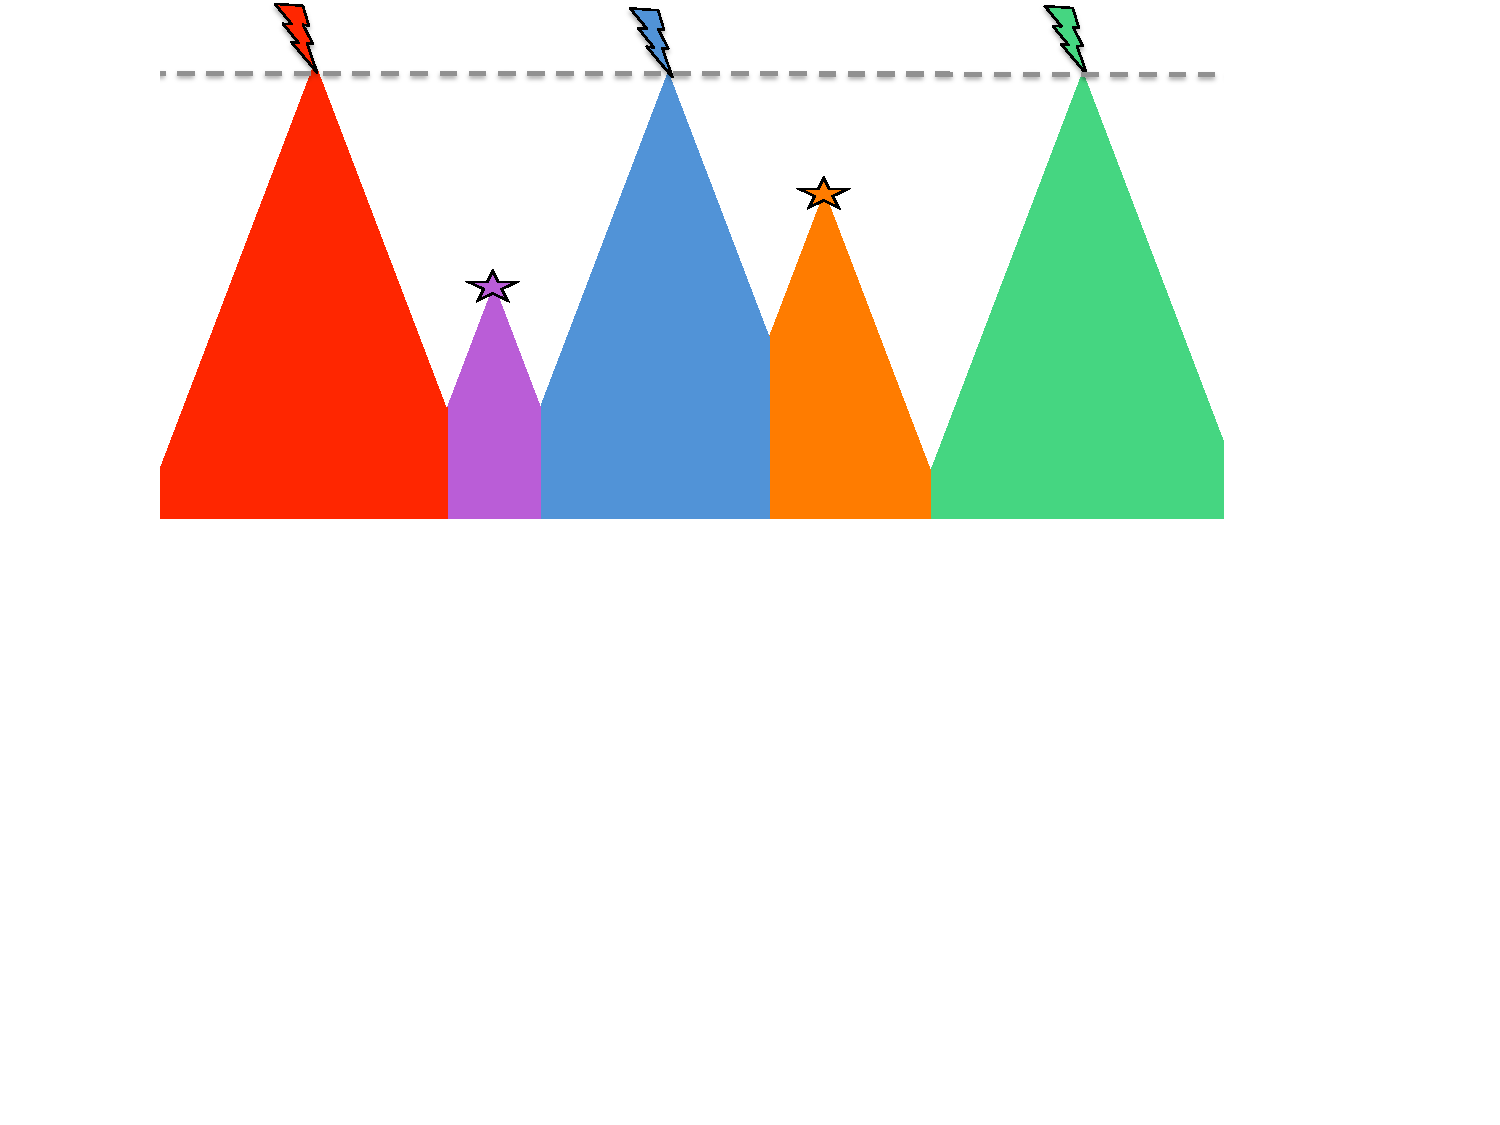
\includegraphics{spreading_alleles_trimmed}
  \end{center}
  \caption{
{\bf Cartoon space-time diagram of the geographic spread of standing and new mutations}. Time
runs down the page, and a single spatial dimension runs across the
page. The environment switches at $t=0$, and following that adaptive
alleles that are successful, at escaping loss by drift, spread from
standing variants (lightning bolts) and new mutations (stars). 
The mean spatial density of successful standing variants at $t=0$ is $\lambda_0$,
and the mean density in space $\times$ time of successful new mutations is $\lambda$.
Our successful alleles spread spatially outwards at speed $v$ and hence carve
space-time cones in previously unadapted areas. When our adaptive
alleles meet their rapid advance is halted due to them selectively
excluding one another, and so their boundaries form straight lines on
short time-scales (overly longer time-scales they will mix into each
other). The grey dashed line shows a cone radiating backward in space-time,
originating from a point $(x,t)$, with slope $v$, its radius at $t=0$
is $v t$. Any successful new allele that arose within this backwards
pointing cone, and any successful standing variant present on the base of this cone, would have spread to $x$ by time $t$.
}
  \label{fig:cartoon}
\end{figure}


%%%%%%%%% %%%%%%%%%%%

\subsection{G6PD example}

Below we describe a number of properties of our process, but we will first introduce 
a motivating example to provide some concrete
numbers to use for illustrative purposes.

Over roughly the past ten thousand years, alleles conferring resistance to malaria have arisen in a number of genes 
and spread through human populations in areas where malaria is endemic \citep{Kwiatkowski:05}. 
A number of these alleles appear to be examples of convergent adaptation, 
as different derived mutations in the same gene are seen in different individuals.
For example, 
a number of changes that confer malaria resistance have been observed in the $\beta$-globin gene;
and the sickle cell allele may plausibly have arisen by up to five independent occurrences
of the same base pair mutation at different locations within Africa
\citep{Flint:98,ralphcoop2010}.
Another particularly impressive case of convergent evolution in response to
selection pressures imposed by malaria are the numerous changes throughout the X-linked G6PD gene, 
with upward of 50 polymorphic variants (above $1\%$ local frequency) having so far been described 
that lower the activity of the enzyme \citep{Howes-g6pd-variants,Minucci-g6pd}. 
These alleles are now found at a combined frequency of around 8\% frequency in malaria endemic areas,
rarely exceeding 20\% \citep{Howes-g6pd-preval}. 
Whether these all confer resistance to malaria is unknown,
but malaria is thought to be the primary driver of these polymorphisms
\citep[see][ for a general review]{hedrick2011population}.
Three G6PD deficiency alleles are particularly common and relatively well studied: 
the $A-$ allele found in much of sub-Saharan Africa; 
the Med allele found in the Mediterranean and Middle East; 
and the Mahidol allele found Myanmar and Thailand.
The $A-$ and Mahidol alleles have been shown
to be protective against {\it Plasmodium falciparum} and {\it P.\ vivax} in both
hemizygote males and both heterozygote and homozygotes females \citep{Ruwende-g6pd, Louicharoen-g6pd}. 
Haplotype-based analysis of genetic diversity surrounding
$A-$, Med, and Mahidol suggest that they have spread over the past 
few thousand years \citep{tishkoff-g6pd,Slatkin-age-est,Saunders-g6pd,Louicharoen-g6pd}, 
consistent with the age of other known malaria resistance alleles. 
Population genetic analyses suggest that these three variants each have a hemizygote/heterozygote 
selection coefficient of $0.05-0.3$
\citep{tishkoff-g6pd,Slatkin-age-est,Saunders-g6pd,Louicharoen-g6pd}. 
This is in reasonable agreement with the selection coefficients calculated by
\citet{Ruwende-g6pd} on the basis of the present day levels of
resistance to malaria due to the $A-$ allele. \\

Given such a strong pressure on these alleles they should have risen
quickly to fixation, so their presence at intermediate frequency,
over a broad geographic area, makes it a good candidate for a recently
balanced polymorphism due to heterozygote advantage \citep[note that
the conditions for a balanced polymorphism are
complicated by the hemizygosity of males, see][]{hedrick2011population, Pamillo:1979}. 
Indeed, hemizygous males and homozygous females suffer from G6PD deficiency,
leading to hemolytic anemia when exposed to a variety of compounds, notably
those present in fava beans (although, It is unclear if this alone is enough of a
selection pressure to maintain the polymorphism in the face of these alleles
considerable malaria resistance advantage). 
The theory we use regarding the ``wave of advance'' \citep{fisher1937wave}
applies as well in the case of heterozygote advantage
\citep{aronson1975nonlinear}, with the selected allele spreading
locally to the equilibrium frequency (rather than fixation). 
Therefore, our framework is applicable to the spread of G6PD, with speed determined by the advantage of heterozygotes when rare.
We assume that before malaria became prevalent, 
G6PD deficiency alleles suffered a decrease in relative fitness of $s_d$ in heterozygote and homozygotes females and hemizygote males. 
Assuming that the underlying causes and strength of this drop in fitness have not changed, 
we estimate that $s_d$ has to have been upward of $\sim 0.05$ (if $sb
\geq 0.05$),
in order to have resulted in the equilibrium frequency seen today in
areas with endemic malaria \citep[see also][]{Ruwende-g6pd}. 

%Hedrick sex-specific review http://www.eeslmu.de/eeswiki/images/Hedrick_Review.pdf
% Fry: http://www.ncbi.nlm.nih.gov/pmc/articles/PMC3654548/
% kidwell http://www.ncbi.nlm.nih.gov/pmc/articles/PMC1213615/
%Rice: http://www.jstor.org/discover/10.2307/2408385?uid=3739560&uid=2129&uid=2&uid=70&uid=4&uid=3739256&sid=21103992458511



% G6PD frequency across world http://www.google.com/imgres?imgurl=http%3A%2F%2Fwww.plosmedicine.org%2Farticle%2Finfo%3Adoi%2F10.1371%2Fjournal.pmed.1001339.g002%2Flargerimage&imgrefurl=http%3A%2F%2Fwww.plosmedicine.org%2Farticle%2Finfo%253Adoi%252F10.1371%252Fjournal.pmed.1001339&h=2938&w=2381&tbnid=oD_tX3ea8IbLfM%3A&zoom=1&docid=k37axqAZDS7ljM&ei=5rdOU5TVDMqj8QGntICYBg&tbm=isch&ved=0CF8QMygLMAs&iact=rc&uact=3&dur=1447&page=1&start=0&ndsp=15

% Spatial distribution of G6PD alleles:  http://www.malariajournal.com/content/12/1/418

%IDEA: could we look at all freq. reports of g6pd and see if male and
%female freq. diffs support model of sexual-conflict?

The geographic area of Central and Eastern Asia with malaria is 
on the order of ten million square kilometers.
In that area there are at least $15$ common variants \citep[see Figure \ref{fig-G6PD-map}][]{Howes-g6pd-variants}. 
Therefore, the average width of an area occupied by an allele is $\sqrt{10^7/15} \approx  800$km. 
The coding region of G6PD is 515 codons long, 
and around 140 distinct deficiency alleles have been observed. 
Assuming a mutation rate of $\approx 10^{-8}$ per base pair per generation, 
we can take as an order-of-magnitude estimate $\mu \approx 1 \times 10^{-6}$ per generation. 
The dispersal and demographic parameters of humans in the past few thousand years is unclear,
particularly as we are concerned with the ``effective'' population density
(i.e.\ population density divided by variance in offspring number).
We therefore will use two reasonable values for the effective population density: $\rho=2$ and $0.2$ people per km$^2$,
and three values for the dispersal distance: $\sigma=10$, $50$ and $100$ kilometers per generation.
Clearly, human migration has been shaped both by local dispersal and larger-scale expansions 
\citep[see][for a recent discussion]{Pickrell:14}, 
so these parameters only provide a rough view of the process.

\begin{figure}[ht]
\begin{center}
  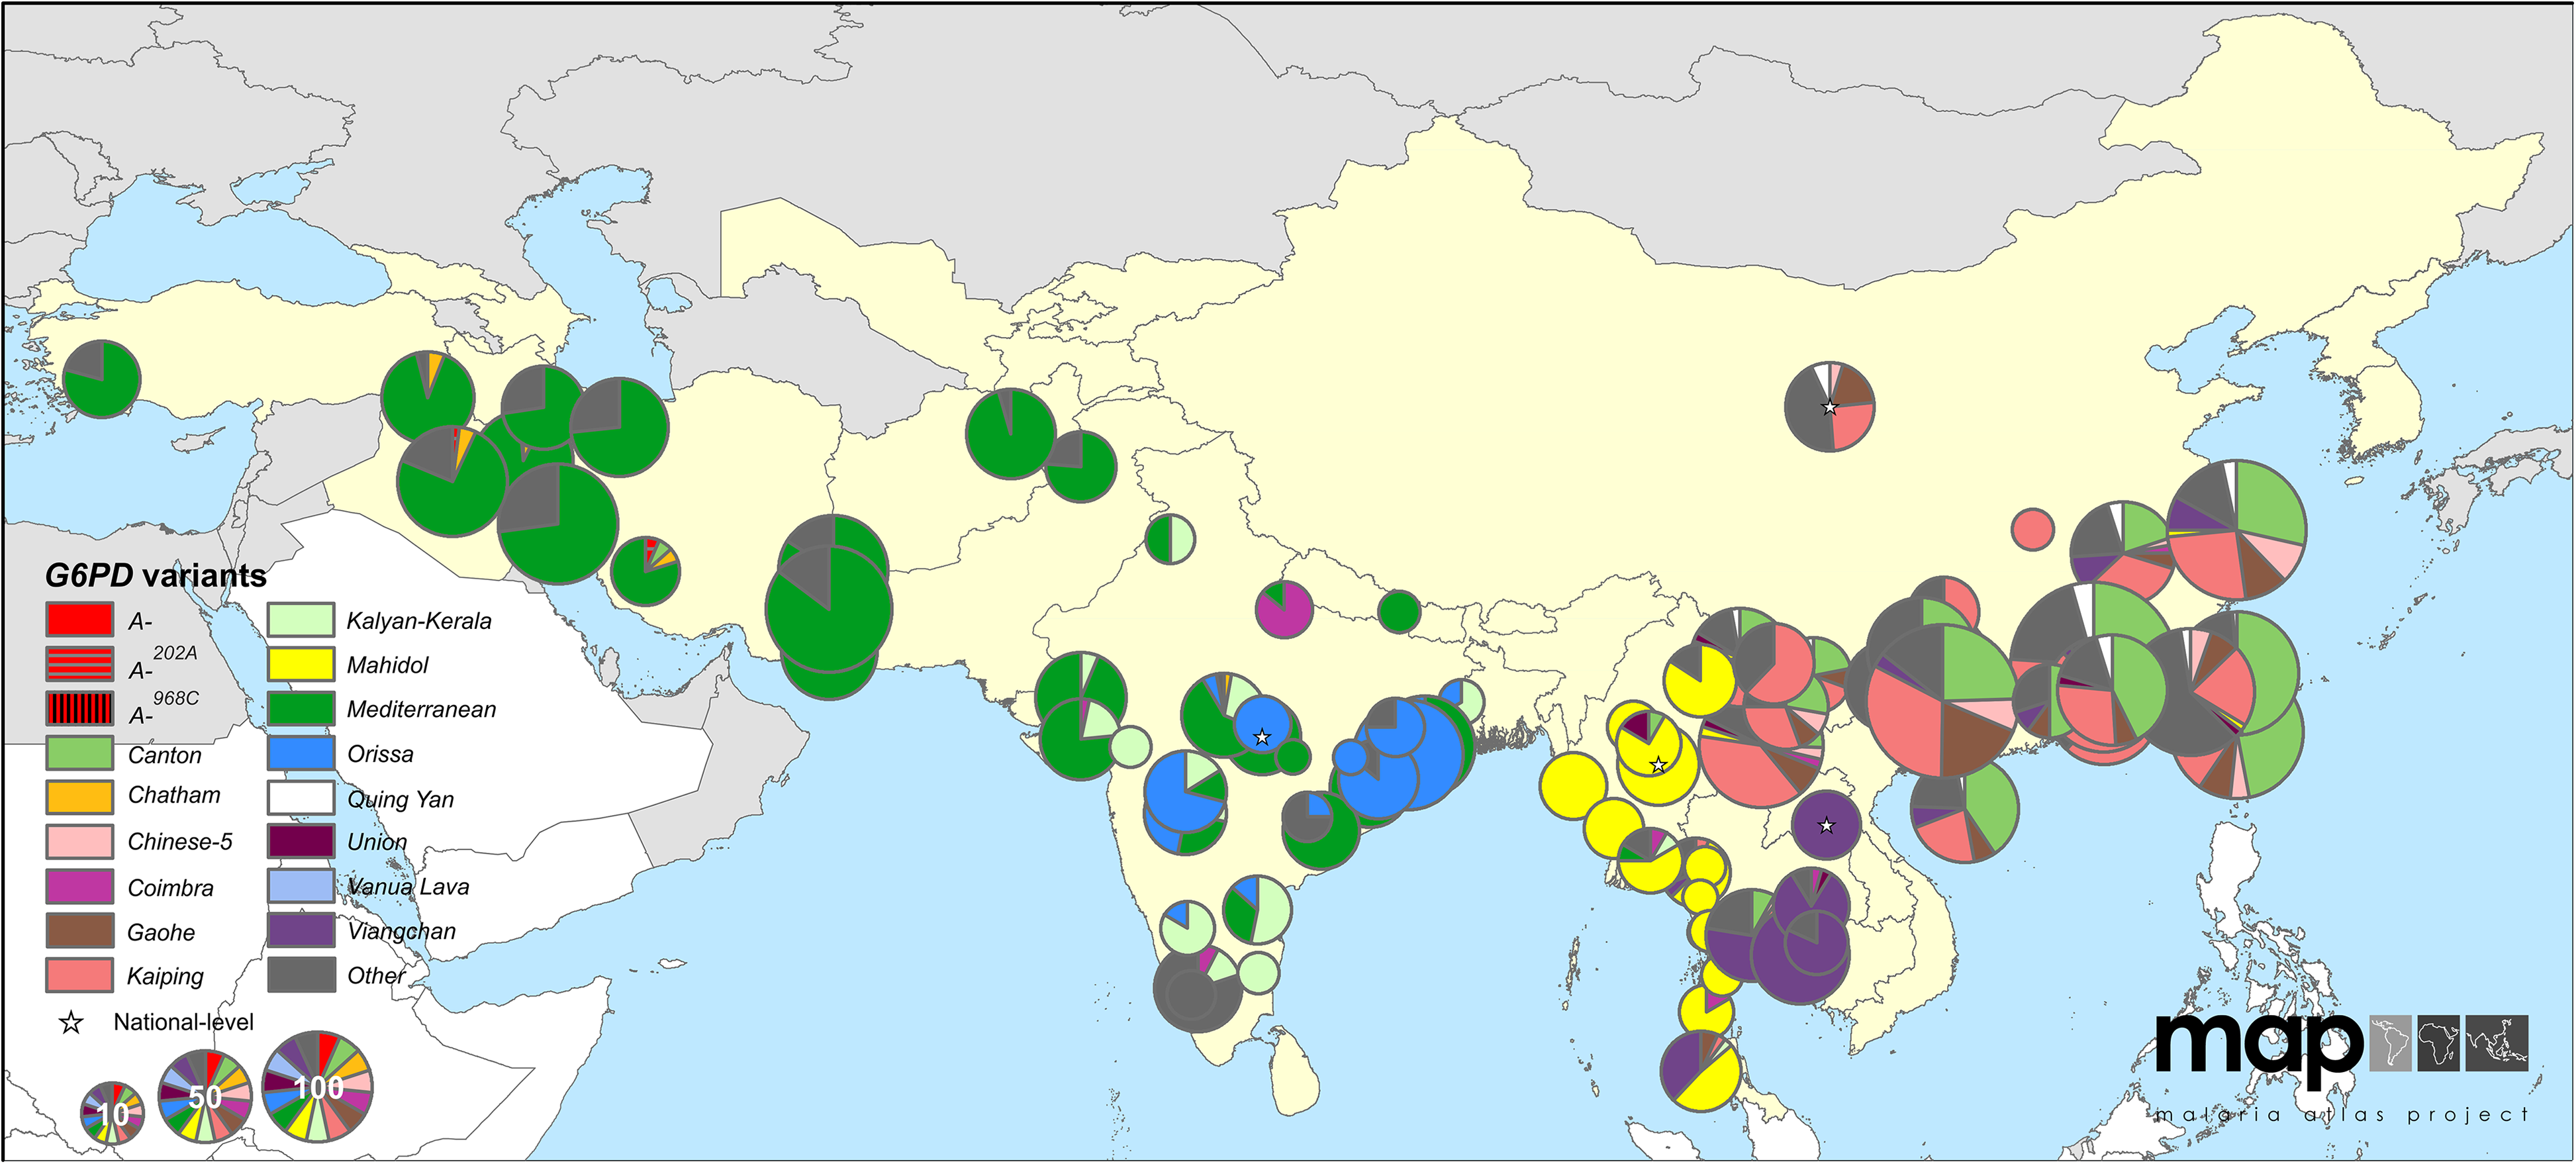
\includegraphics[width=1.0\textwidth]{G6pd_Howes_et_al_1475-2875-12-418-4}   %{charlen-by-sd-limit}
\caption{ 
{\bf Map of G6PD-deficiency allele frequencies across Asia.} 
The pie chart shows the frequency of G6PD-deficiency alleles. 
The size of the pie chart indicates the number of G6PD-deficient individuals sampled.
Countries with endemic malaria are colored yellow. 
Figure taken from \citet{Howes-g6pd-variants}
\url{http://www.malariajournal.com/content/12/1/418}. 
} \label{fig-G6PD-map}
\end{center}
\end{figure}

% \begin{figure}[ht]
% \begin{center}
%   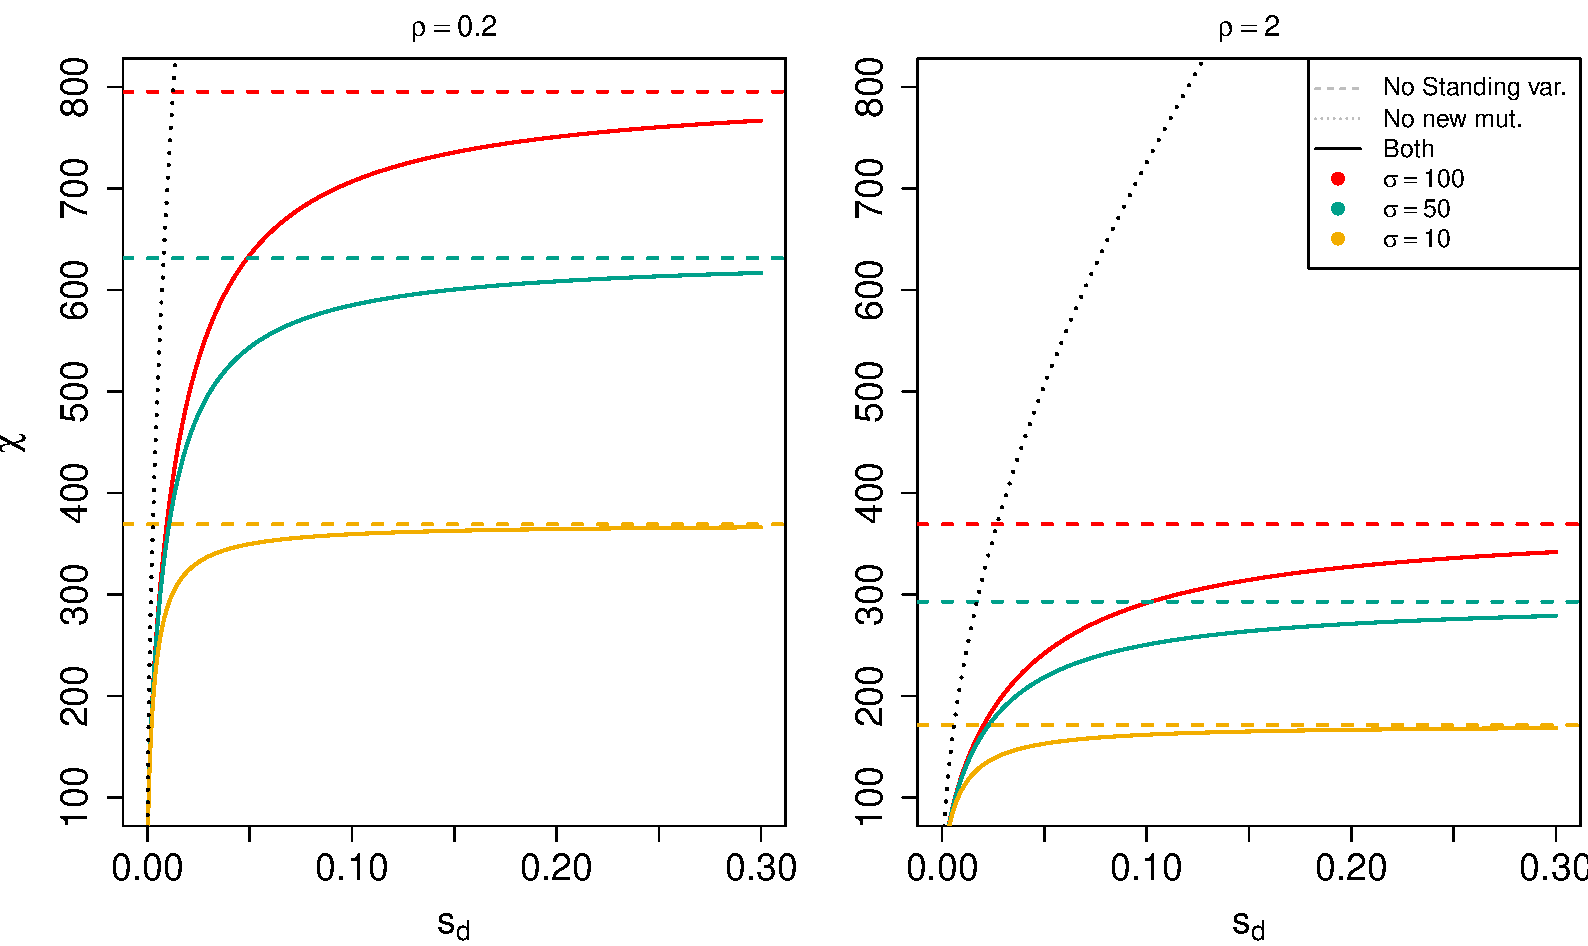
\includegraphics[width=1.0\textwidth]{G6PD_charlengths}
% \caption{ %
% {\bf Characteristic length,} as a function of dispersal distance $\sigma$ and selective disadvantage $s_d$.  XXX at what parameters. XXX
% } \label{Fig-G6PD-charlength}
% \end{center}
% \end{figure}

%$A-$ ?? risk lower of severe malaria for both female heterozygotes and male
 %hemizygotes estimates of selection pressure \citep {Ruwende-g6pd}
%Mahidol487A \citep{Louicharoen-g6pd}
%Show's effect in het and homozy females


%Selection coefficient (s) 	A- 0.044 (0.019–0.048)  Med	0.034
%(0.014–0.049)  ``The mean age of the A- allele in these runs was 6357 years, with a 95\% credibility interval extending from 3840 to 11,760 years. For the Med alleles, the mean age was 3330 years with a 95\% credibility interval of 1600 to 6640 years"
%\citet{tishkoff-g6pd}
%s 0.24 and t= 40 generations \citep{Slatkin-age-est}
%The estimated age is ~100 generations with an upper bound of <150
%generations A- 0.1 < s < 0.2 \citep{Saunders-g6pd}
%Mahidol487A mutation started to increase at ~1500 YBP, with a
%selection intensity of ~0.23 \citep{Louicharoen-g6pd}
%Shows effect in het and homozy females


%%%%%%%%%%%% %%%%%%%%%%%%%%%

\subsection{The geographic resolution of adaptation from new and standing variation}

% a characteristic length of regions and a proportion of haplotypes (or of space?) that are from standing variation

In \citet{ralphcoop2010}, studying the model without standing variation,
we defined a {\em characteristic length} which gave the spatial scale across which mutants with distinct origins would establish.
This was proportional to the mean distance between neighboring established mutants,
but had the advantage of being easier to calculate.
Furthermore, the time scale over which adaptation occurred could be found by dividing the characteristic length 
by the speed at which the mutants spread.
We first define a similar characteristic length for this new model. %,
%as well as a similar compound parameter describing the relative importance of standing variation to the process of adaptation.
%(Note that a similar approach, summarizing with a {\em characteristic length} was taken by \citep{slatkin1973geneflow} for a different problem.)

Suppose we fix our attention on a particular new mutation that happens to be the first to occur in some region.
If it does not encounter other locally fixed, beneficial mutants,
it will cover a distance $L$ in time $L/v$.
The number of other mutations appearing in the circle it has covered up until this time is Poisson with mean
$\lambda_0 \pi L^2 + \lambda \pi L^3 /v$ in two dimensions
(and $2 \lambda_0 L + 2 \lambda \pi L^2 /v$ in one dimension).
% $\lambda_0 \omega_d L^d + \lambda \omega_d L^{d+1} /v$ in $d$ dimensions
Therefore, if we define $\chi$ for a two-dimensional model to be the unique positive solution to
\begin{equation}
    \lambda_0 \pi \chi^2 + \lambda \pi \chi^3 /v = 1,
\end{equation}
then $\chi$ gives the distance spread unobstructed by the descendants of a new mutant
before it is expected that one other successful mutation would have arisen in the area covered so far.
The explicit formula for $\chi$ in two dimensions is cumbersome; here we omit it.
(In one dimension the characteristic length is $\chi = ( \sqrt{\lambda_0^2 + 2 \lambda/v} - \lambda_0 )/( 2 \lambda / v )$.)
Substituting expressions for $\lambda_0$, $\lambda$, and $v$ from above,
we can rewrite this as
\begin{equation} \label{eqn:defines_chi}
%    \left( \frac{ - \chi \log(1-s_d) }{ 2 s_b \sigma } \right)^2 + \left( \frac{ - \chi \log(1-s_d) }{ 2 s_b \sigma } \right)^3 
%        = \frac{ - \log(1-s_d)^3 }{ 4 s_b^2 \sigma^2 \pi \rho \mu } .
   \frac{\sqrt{2s_b} }{-\log(1-s_d) } \chi^2 + \frac{1}{\sigma} \chi^3 = \frac{1}{\sqrt{2s_b} \rho\mu\pi}
\end{equation}
From this we see that $\chi$ decreases with $\rho$ and $\mu$.
Furthermore, for large $\sigma$, the characteristic length is close to the value obtained just from standing variation:
\begin{equation} \label{eqn:chi_standing}
\chi = \sqrt{ -\log(1-s_d) / 2 s_b \rho \mu \pi } + O(1/\sigma).
\end{equation}
On the other hand, if the mutant allele is highly deleterious before $t=0$,
then the characteristic length is close to the value from \citet{ralphcoop2010}:
\begin{equation} \label{eqn:chi_new}
\chi = ( \sigma / \rho \mu \pi \sqrt{2 s_b} )^{1/3} + O(1/\log(1-s_d)).
\end{equation}
These two end points help build our intuition for the interaction of
parameters in shaping the geographic scale of convergent evolution.
By the above calculation, we know that the relevant mutations occur about distance $\chi$ apart, 
 and occur within the first $\chi/v$ generations.
 Said another way, if we look in a circular region of space of radius $\chi$ over $\chi/v$ generations,
 we expect to find roughly one mutational origin.

%XXX could do calculations as in "panmixia" here, e.g.\ if $f = (\chi \sqrt{\pi \lambda_0})^2$ then
%$f = 1-\gamma f^{3/2}$, where
%$\gamma = (4 \pi^{5/2} / \sqrt{2}) \mu^2 s_b^{3/2} \rho^2 / \sigma \log(1/(1-s_d))$.
%Then if $\gamma \ll 1$, $f \approx 1$, while if $\gamma \gg 1$, then $f \approx 0$.

%%%GRAHAM: I commented this out. We return to do proportion standing
%%%below, so perhaps nicer to restrict that to one place. 
% By the above calculation, we know that the relevant mutations occur about distance $\chi$ apart, 
% and occur within the first $\chi/v$ generations.
% Said another way, if we look in a circular region of space of radius $\chi$ over $\chi/v$ generations,
% we expect to find one mutational origin;
% we denote the probability that this mutation is from standing variation by $\pi_0$.
% Therefore, $\pi_0$ is roughly the proportion of establishing mutations that come from standing variation,
% and it is an property of competing Poisson processes that
% \begin{align} \label{eqn:pizero}
%     \pi_0 = \lambda_0 \pi \chi^2 .
% \end{align}
% (In one dimension, $\pi_0 = 2 \lambda_0 \chi$.)


In Figures \ref{Fig-G6PD-charlength} and \ref{Fig-G6PD-charlength-sb} we show the range of characteristic lengths as a function 
of various parameters chosen to match the evolution of malaria
resistance at G6PD. 
These curves match our intuition that population densities result in
smaller characteristic lengths (as would higher mutation rates). 
Allowing standing variation increases the mutational
input and so decreases the characteristic length below that predicted
by only new mutations (i.e.\ equation \eqref{eqn:chi_new}, \citet{ralphcoop2010}).
In turn, increasing the prior deleterious effect of the allele ($s_d$)
acts to increase the
characteristic length until it reaches that predicted by new mutation alone. 
Higher dispersal distances lead to larger characteristic lengths, 
since more rapid geographic spread blocks others from arising. 
A larger selective advantage ($s_b$) acts in two conflicting
ways: aiding the rapid geographic spread of established alleles, and also helping more independent copies
escape drift and become established. 
The effect of helping establish alleles wins out, since increasing the selective benefit $s_b$ decreases the characteristic length. 
 (This can be shown in general by differentiating \eqref{eqn:defines_chi} with respect to $z=\sqrt{s_b}$,
showing that $\partial_{z} \chi = - ( C_1 z \chi + C_2 \chi^2 )/(C_3 z^2 + C_4 z \chi ) \le 0$ for appropriate nonnegative constants $C_{1--4}$.) 
This effect is strongest when only standing variation contributes ($s_b^{-1/2}$, equation \eqref{eqn:chi_standing}), 
as in that case the speed of spread does not matter. 
The dependence of the characteristic length on $s_b$ when only new mutations contribute is much weaker ($s_b^{-1/6}$, equation \eqref{eqn:chi_new})
Overall, the range of characteristic lengths observed are reasonably
consistent with the average diameter of a G6PD variant in Eurasia of
800km, especially for the lower population density, as long as the
fitness cost of G6PD-deficiency alleles before malaria ($s_d$) was not too low. 

\begin{figure}[ht]
\begin{center}
  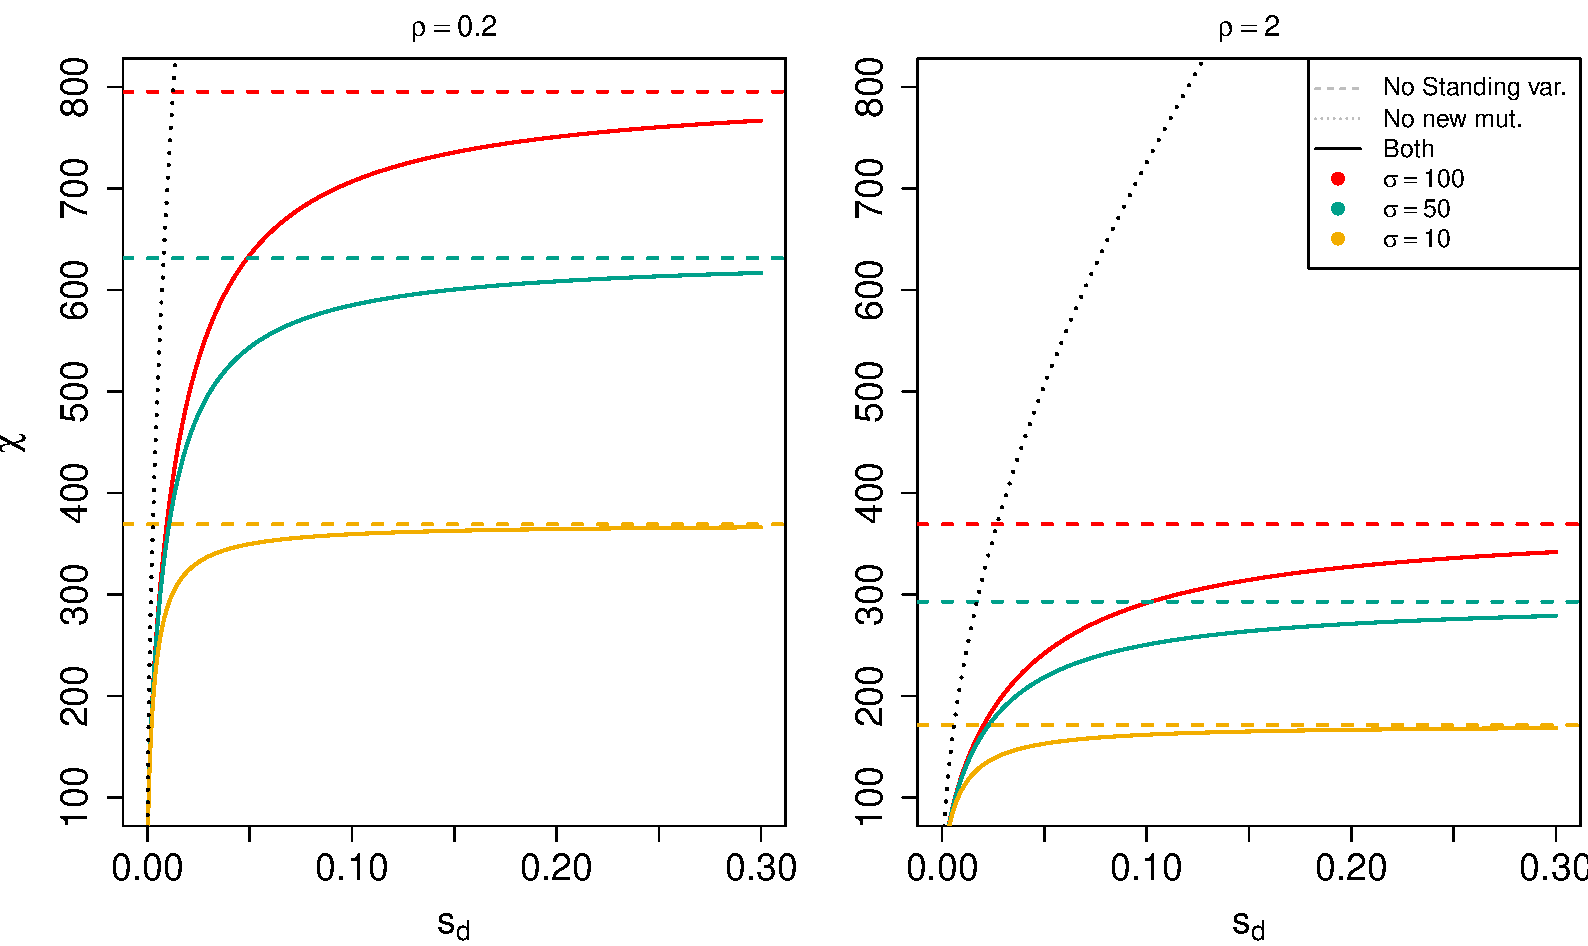
\includegraphics[width=1.0\textwidth]{G6PD_charlengths}   %{charlen-by-sd-limit}
\caption{ %
{\bf Characteristic length, as a function of selective disadvantage}, 
compared to the corresponding quantity without standing variation (equation \eqref{eqn:chi_new}) 
and to the quantity only considering standing variants (equation \eqref{eqn:chi_standing}).
The other parameters are chosen to match those of G6PD,
$\mu = 10^{-5}$ and $s_b = 0.05$. As the characteristic length with
only standing variation is independent of dispersal distance it is
plotted as a single black dotted line. 
} \label{Fig-G6PD-charlength}
\end{center}
\end{figure}

\begin{figure}[ht]
\begin{center}
  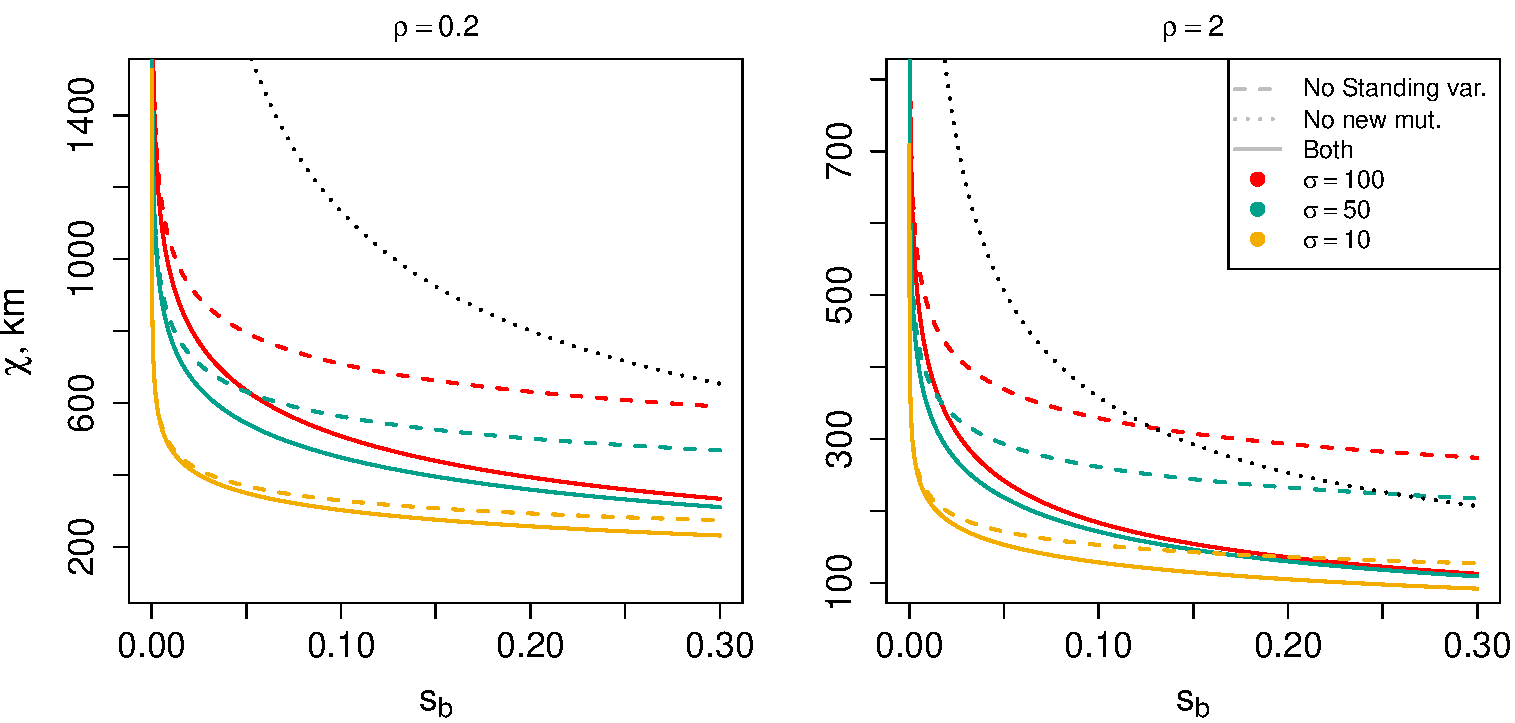
\includegraphics[width=1.0\textwidth]{G6PD_charlengths_sb}   %{charlen-by-sd-limit}
\caption{ %
{\bf Characteristic length, as a function of selective advantage},
holding the prior disadvantage of the allele fixed at $s_d=0.05$ and the mutation rate fixed at $\mu=10^{-5}$.  
We compare this to the corresponding quantity without standing
variation (equation \eqref{eqn:chi_new}) 
and to the quantity only considering standing variants (equation \eqref{eqn:chi_standing}).
} \label{Fig-G6PD-charlength-sb}
\end{center}
\end{figure}


% \begin{figure}[ht]
% \begin{center}
%   \includegraphics[width=1.0\textwidth]{charlen-by-sd-sigma}
% \caption{ %
% {\bf Characteristic length,} as a function of dispersal distance $\sigma$ and selective disadvantage $s_d$.  XXX at what parameters. XXX
% }
% \end{center}
% \end{figure}

%%%%%%%%%%% %%%%%%%%%%%%% %%%%%%%%%
\subsection{Time to adaptation}

It is also straightforward to compute the mean time until adaptation.
Imagine ourselves at some geographic location, and let $\tau \ge 0$ be the time at which we are first reached by some advantageous mutation.
Then, as can be seen from the
perspective of the grey dot in Figure~\ref{fig:cartoon}, 
$\tau > t$ if and only if the cone with point at $(x,t)$ and slope $v$
extending back to $t=0$ (light grey dashed lines) is empty of successful mutations.
Since we assume these are a Poisson process, 
in two dimensions
\begin{equation} \label{eqn-no-mut-t}
    \P\{ \tau > t \} = \exp\left( - \lambda_0 \pi v^2 t^2 - \lambda \pi v^2 t^3 / 3 \right) ,
\end{equation}
i.e. the combined probability that area of a circle of radius $vt$ surrounding our
point at $t=0$ was free of successful standing variants, and no
successful, new mutations arose in the cone (that has radius $r=vt$ at
$t=0$ and height $h=t$, and hence volume $\pi r^2 h/3$). 
Since $\E[\tau] = \int_0^\infty \P\{ \tau > t \} dt$,
\begin{align}
    \E[\tau] % &= \int_0^\infty \P\{ \tau > t \} dt \\
        &= \int_0^\infty \exp\left( - \lambda_0 \pi v^2 t^2 - \lambda \pi v^2 t^3 / 3 \right) dt.
\end{align}
For means of evaluating this integral, see Appendix \ref{apx:integrals}.


In Figure \ref{G6PD_chartimes} we show the mean time until adaptation
for various values of the parameters chosen to match the case of
adaptation at G6PD. Increasing $\sigma$ and decreasing $s_d$ lower 
the time to adaptation, as alleles spread geographically more quickly
and are present as standing variation more often
respectively. Increasing $s_b$ strongly decreases the time to
adaptation, as it both causes more alleles to escape drift and to
rapidly spread. Given that the G6PD alleles likely spread over a few
thousand years, i.e.\ less than a few hundred generations, 
this time scale seems quite plausible, except perhaps for the lowest dispersal distances.  



\begin{figure}[ht]
\begin{center}
  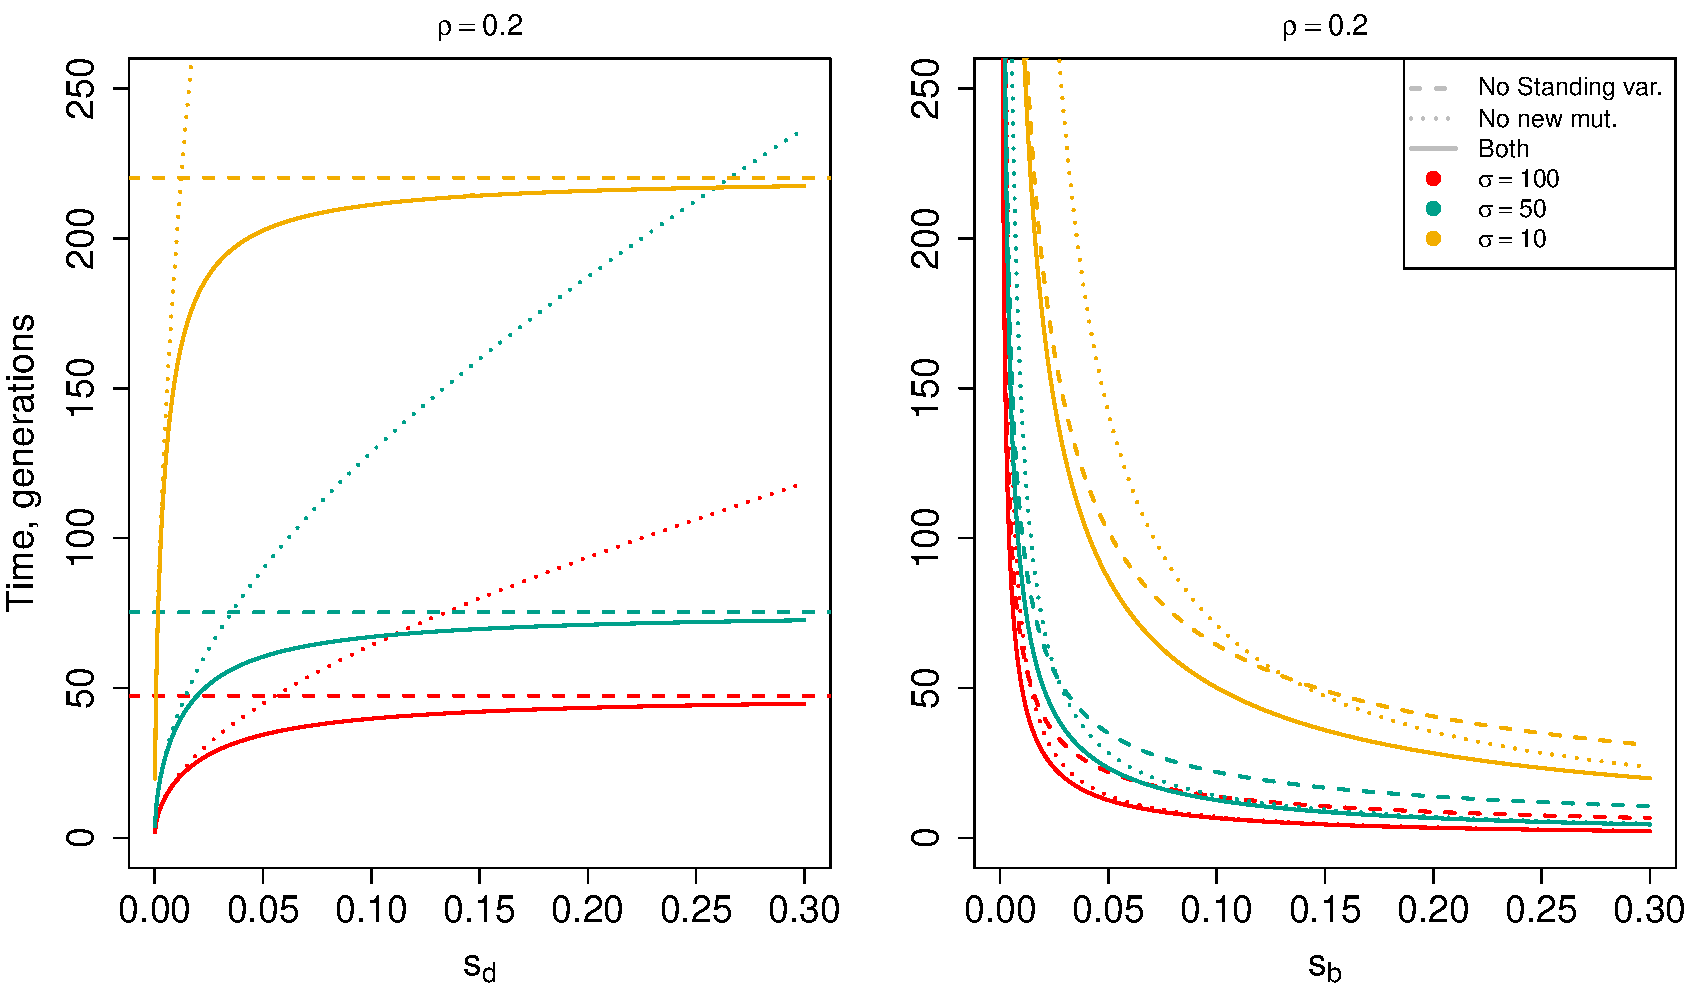
\includegraphics[width=1.0\textwidth]{G6PD_chartimes_sd_sb.pdf}   %{charlen-by-sd-limit}
\caption{ %
{\bf Mean adaptation times}, as a function of selective disadvantage
and , compared to the corresponding quantity without standing variation, and to the quantity only considering standing variants.
} \label{G6PD_chartimes}
\end{center}
\end{figure}

% proportion of haplotypes (and of space) that are from standing variation 

\subsection{The contribution of standing variation.}
We can use our framework to address what proportion of new adaptive variants arise from standing variation.
We have defined $\lambda_0$ to be the mean density
of standing variants that are present and escape loss when the
environment shifts.
We will define $\nu_+$ to be the mean density of newly arising alleles
that spread having arisen in an area free of other adaptive alleles.
Since the probability that a mutant arising at location $x$ and time $t$ 
is lucky enough to be born in a location not already occupied by mutants
is $\P\{ \tau > t \}$,
we can see  $\nu_+ = \int_0^\infty \lambda \P\{\tau>t\} dt$, and hence
$\nu_+ = \lambda \E[\tau] $.
Using that $\lambda_0 = \lambda / \log(1/(1-s_d))$, this gives us that
\begin{equation}
    \nu_+ = (\mbox{mean density of new patches}) = \frac{1}{1-\log(1-s_d) \E[\tau]} .
\end{equation}
Therefore, the mean proportion of patches that come from standing variation
is 
\begin{equation} \label{prop_patches_standing}
\lambda_0 / (\lambda_0 + \nu_+) .
\end{equation}
% this gives us the exact quantity we approximated by $\pi_0$ in \eqref{eqn:pizero}.
There are $\lambda_0 + \nu_+$ patches per unit area, so
the typical patch (i.e.\ with distribution given by the Palm measure) occupies area $1/(\lambda_0 + \nu_+)$.

We can also find the mean proportion of space covered by standing
variants (we will restrict ourselves to two dimensions).
At time $t$ a geographic location has not yet been reached by the
mutation with probability given by equation \eqref{eqn-no-mut-t}.
The probability, given that it has not been reached by $t$, that it will be reached by time $t+dt$ 
by a standing variant is approximately $2 \lambda_0 \pi v^2 t dt$,
which is $\lambda_0$ multiplied by the thin slice of extra area in our
expanded circle at $t=0$, which has gone from a radius $vt$ to
$v(t+dt)$. The corresponding probability the point is reached by a new
variant is 
$\lambda \pi v^2 t^2 dt$, which is $\lambda$ multiplied by the
sliver of  extra volume in our space-time cone at time $t+dt$ compared to that at time $t$.
Therefore, as is standard for competing exponentials,
the probability a given location is reached first by a standing variant,
and therefore the mean proportion of space covered  by standing variants,
is
\begin{equation} \label{prop_space_standing}
    z_0 = \int_0^\infty {2 \lambda_0 \pi v^2 t} \; \exp \left( - \lambda_0 \pi v^2 t^2 - \lambda \pi v^2 t^3 / 3 \right) dt .
\end{equation}
To evaluate this integral, again see Appendix \ref{apx:integrals}.
%\marginnote{put in this value in terms of Gaussian CDF?}

Furthermore, if we define $a_0$ to be the mean area occupied by a typical standing variant, 
then $a_0$ is given by the proportion of the range occupied by standing variants divided by the mean density of unique standing variants,
i.e.\ $a_0 = z_0 / \lambda_0$.
We can solve for $a_+$, the corresponding mean area occupied by a given new variant, 
using the formula $a_0 / a_+ = z_0 / (1-z_0)$.

In Figure \ref{G6PD_standing_var_proportion} we show the proportion of
alleles that spread from standing variation, and the proportion of
geographic space covered by standing variants for parameters chosen to match our G6PD example.
Even for relatively large deleterious costs prior to the environmental
switch standing variants still makes up quite large proportion of the
adaptive alleles, and an even larger proportion of the range (as they
get to occupy a larger area than new mutations, as they start earlier).

\begin{figure}[ht]
\begin{center}
  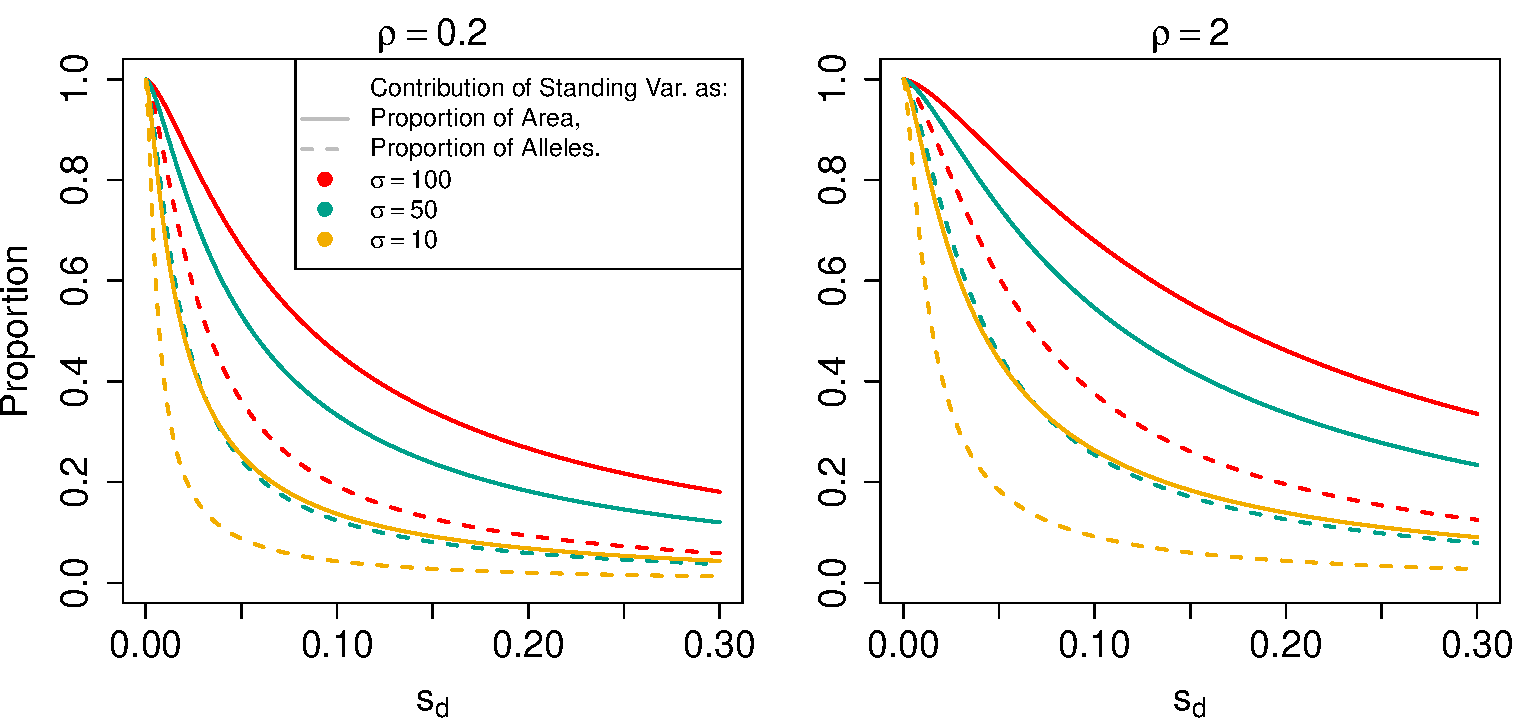
\includegraphics[width=1.0\textwidth]{G6PD_standing_var_proportion}
\caption{ %
{\bf Mean proportion of patches arising from standing variation.} The
parameters given are for the G6PD example.
The left and right panels show the expected proportion of patches that
arise from standing variation and the expected proportion of
geographic space that is covered by adaptation from standing variation
(equation \eqref{prop_patches_standing} and \eqref{prop_space_standing} respectively).
We set $\mu=10^{-5}$ and $s_b=0.05$ to match our G6PD example.} \label{G6PD_standing_var_proportion}
\end{center}
\end{figure}


%{\tt Simulations:} 
%compare mean density against $s_d$ at different values of $\sigma$; 
%omit variability if needed for readability. 
%Compare to panmictic results.


\subsection{Multiple variant types}
Another problem that we can seek to address with this work is
the extent to which pleiotropy biases 
adaptation towards the repeated use of particular subset of loci
(i.e.\ convergence at genetic level). 
While many alleles may confer the beneficial phenotype, 
not all will contribute equally to adaptation if they have negative pleiotropic consequences.
There are at least two ways that negative pleiotropy can contribute to high rates of convergence 
when adapting if a single change is sufficient for adaptation. 
First, negative pleiotropic effects can reduce 
the overall beneficial selection coefficient of an allele in the new environment,
making them unlikely to become established and slow to spread 
(and in the worst case making them deleterious). 
This first effect has been well studied by a number of authors
\citep{Orr:00,Otto:04,WelchWaxman:03,Chevin:10} and its role in precise genetic
convergence examined \citep{Orr:05,Chevin:10,Unckless:09}. 
A second contribution is that alleles that have
less negative pleiotropy are more likely to be present as standing variation 
before the environmental shift, and so are more able to respond
immediately.

Here we focus primarily on the second effect. 
Let's imagine for the moment that all classes of beneficial allele 
have the same beneficial selection coefficient. 
Or, at least that beneficial selection coefficients are similar enough that our selective exclusion
approximation holds over the time scale on which we examine the process.
Each class of mutations $j$ has its own mutation rate $\mu_j$ and selective disadvantage $s_{d,j}$ prior to the environmental switch. 
As they have the same beneficial selection coefficient after the switch, 
all of the waves travel outward at a rate $v$. 
Then, the density of type $j$ standing variants per unit area 
and the input rate of \textit{de novo} variants per unit area per generation are, respectively,
\begin{align}
  \lambda_{0,j} = \frac{ 2 \mu_j \rho s_b }{ -\log(1-s_{d,j}) } \qquad \text{and} \qquad    \lambda_{j} = 2 \mu_j \rho s_b .
\end{align}
Using these rates, and an argument analogous to that used to derive
equation \eqref{prop_space_standing},
at the time when every location has been reached by an adaptive allele,
the proportion of the species range covered by alleles of type $j$ is
\begin{equation} \label{eqn-prop-space-allele-j}
    p_j = \int_0^\infty  \left( 2 \lambda_{0,j} \pi v^2 t +  \lambda_j \pi v^2 t^2 \right)  
    \; \exp \left( - \sum_k ( \lambda_{0,k} \pi v^2 t^2 + \lambda_k
      \pi v^2 t^3 / 3 ) \right) dt .  %%deleted \lambda_j \pi v^2 t^3
                                %%out of term out front
\end{equation}
If we only allow standing variation this collapses to 
\begin{equation}  \label{eqn-prop-space-allele-j-standing-room-only}
    p_j = \frac{  \mu_j / \log(1-s_{d,j}) }{\sum_k  \mu_k / \log(1-s_{d,k}) } ,
\end{equation}
while if we only allow new variation, 
i.e.\ if all variants are highly deleterious before the environment switches, 
 $p_j =\mu_j / (\sum_k  \mu_k)$.

To illustrate some of the properties of this model, 
let's imagine the somewhat extreme scenario that there is a single base pair 
at which a possible mutation is relatively free of negative pleiotropy (call this class $1$);
and a larger mutational target where changes 
have more serious pleiotropic consequences in the ancestral environment (class $2$). 
We set $s_{d,1} \leq s_{d,2}=0.05$ and $\mu_1=1 \times 10^{-8}$, 
assume that both classes share a beneficial selection coefficient of $s_b=0.05$,
and think of the second class of alleles as arising at one of ten, a hundred, or one thousand base pairs. 
We show the expected proportion of space covered by
the rarer, class $1$ mutations in Figure \ref{fig:pleiotropy_calc}.
Intuitively, the contribution of the rarer mutation decreases as the
mutational target of the second class becomes larger, and as the
difference in the negative pleiotropic consequences of the two classes of alleles decreases. 
The case with standing variation only is the best case scenario 
for the rarer mutation, so its rate of introduction after $t=0$ is necessarily lower. 
However, the standing-variation-only case does seem to provide a
reasonable rule of thumb, especially for parameter combinations, 
like higher population densities and high dispersal distances, 
that increase the contribution of standing variation (and similarly for high $s_b$). 

\gc{As discussed above, we could incorporate differences in the beneficial selection
coefficients of the different classes of alleles, to allow for
negative pleiotropic effects acting to surpress the advantage of an
allele once the environment switches (effect one above). One simple way to do
this is to simply replace $s_b$ with $s_{b,j}$ resulting in a class-specific new allele establishment rates ($\lambda_{j}$) and rates of spread ($v_j$).
These then could be used in equation
\eqref{eqn-prop-space-allele-j}. We could imagine our two class model, outlined
above, with class one having the additional advantage of
$s_{1,b}>s_{2,b}$. This would further increase the contribution of the rarer class,
because our rare class would overcome drift more often and spread more
rapidly. However, a straight-forward application of the logic of used
to construct equation \eqref{eqn-prop-space-allele-j},
ignores the fact that classes of alleles with higher $s_b$ is not
completely selected excluded from spreading into geographic areas occupied by alleles with lower
$s_b$. Given enough time the most advantageous type (type 1, in this case) would arise and
spread everywhere, and so if we used different $s_b$s in equation
\eqref{eqn-prop-space-allele-j}, it would only be a short-term approximation to
a longer term dynamic. Even after the initial tessellation has formed the allele 1s would have an selective advantage $\delta s
=s_{b,1}-s_{b,2}$ in areas where allele 2 have already spread, and so
would arise at rate $2\rho \mu_1 \delta s $ in these areas and spread through them at
speed $\sigma \sqrt{\delta s}$. An extension of our Poisson process model could incorporate these
 effects, by thinning the Poisson process of establishing mutations by
 correctly. 
Whether allele $2$ persists would
depend on the linkage arrangements between loci. If the loci of allele
1 and 2 are unlinked, then allele 1 can spread without disrupting
allele 2. However, if they are linked the spread of allele $1$ may
push allele $2$ out of the population. More complicated dynamics,
including spatial Dobzhansky-Muller incompatibilities \citep{,Kondrashov:03,ralphcoop2010}, could ensue if
there are epistatic interactions between the alleles. }

% An extension of this Poisson process model could incorporate these
% effects, thinning out mutations  
% It could be interesting to investigate pleiotropy's combined
% effect of adaptation, through standing variation and rate of spread, by coupling together
% $s_{b,k}$ and $s_{d,k}$ perhaps through Fisher's geometric model.
% Using Fisher's geometric model we could allow $s_{b}$ and $s_d$ to be coupled as a consequence of being an
% the fitness in two related environments of some underlying phenotype
% drawn from a continuous distribution,
% rather than our $k$ discrete classes \citep{Chevin:10}.  

%While it may be of interest to explore this model
%incorporating both effects of negative ple

\begin{figure}[ht]
\begin{center}
  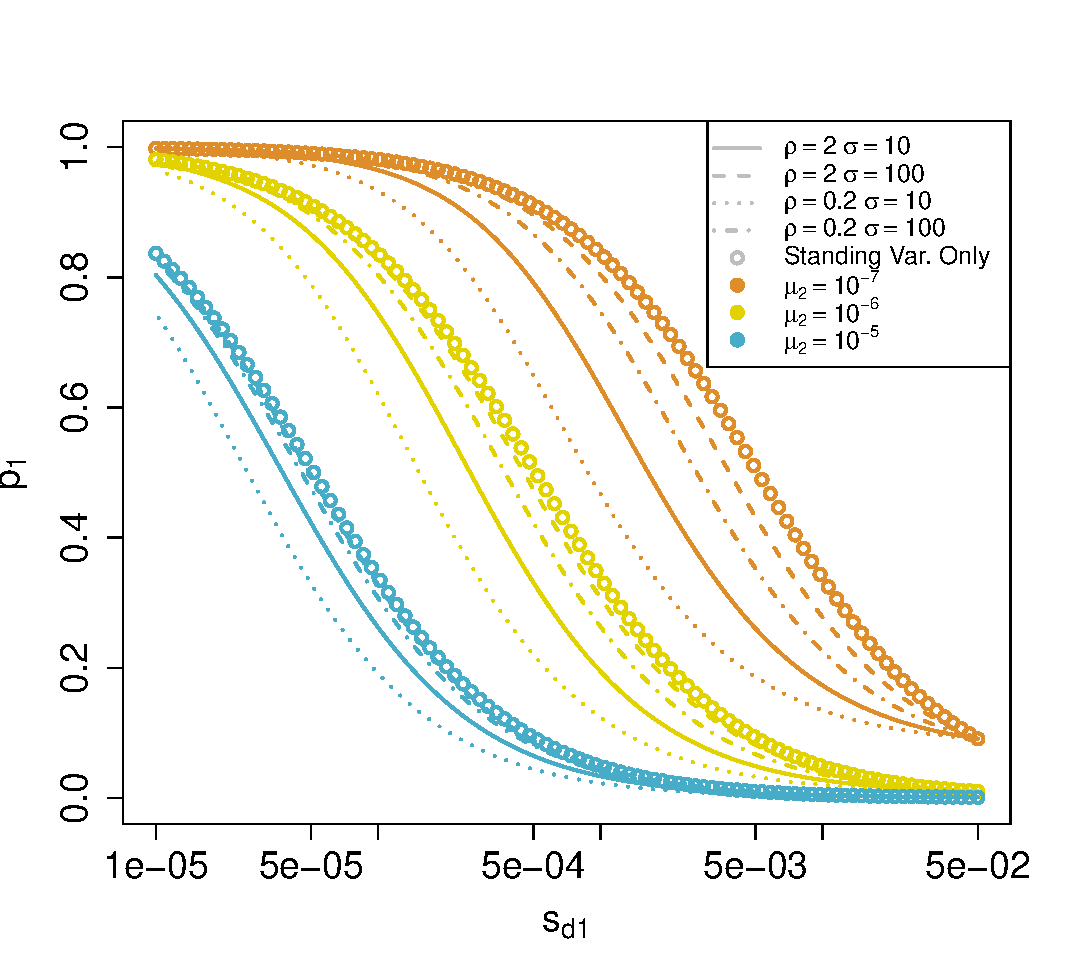
\includegraphics[width=1.0\textwidth]{pleiotropy_calc}
\caption{ %
{\bf Proportion of space covered by rarer but less negatively pleiotropic
  mutation}. Empty circles give the result for standing variation only,
  equation \eqref{eqn-prop-space-allele-j-standing-room-only}. Lines give
  the result allowing both standing and \textit{de novo} mutations (equation \eqref{eqn-prop-space-allele-j}).
  Here we hold $s_b=s_{d,2}=0.05$ and $\mu_1=1 \times 10^{-8}$.
  }   \label{fig:pleiotropy_calc}
\end{center}
\end{figure}


\subsection{Local establishment and comparison to panmixia}

In the above (and in \citet{ralphcoop2010}) we have assumed that once the mutation appears,
conditional on eventual fixation, it begins to spread spatially at speed $v$ instantly,
effectively neglecting the time it must first spend escaping demographic stochasticity.
In \citet{ralphcoop2010} we addressed this by noting that there would be no change at all in our results 
if all mutations had to wait the same amount of time before fixing locally,
and that this time was short relative to the time it took the wave to spread across the characteristic length;
we then showed via simulation that this was reasonable in certain situations.
In this section we examine this assumption in more detail, although mostly through heuristic arguments,
and also compare the results above to the results without geographic structure of \citet{softsweepsII}.

We are assuming that shortly after a new mutation appears, 
it can be approximated by a branching process growing at rate $s$
until the point that it grows large enough to ``feel'' spatial structure,
at which point it begins to spread as a more--or--less deterministic wave.
Although we are not aware of good analysis of this transition, 
the relevant size when spatial structure becomes important
should be something close to $\sigma^2 \rho$ 
(i.e.\ Wright's ``local effective population size'', \citet{Wright:43}).
Let $Z_t$ be a continuous-time branching process with $Z_0=1$ and $\E[Z_t] = e^{s_b t}$.
Then we know that there exists a random variable $W$ such that $\lim_{t\to\infty} e^{-s_b t} Z_t = W$ almost surely,
so that if $\tau$ is the time $Z_t$ reaches size $\sigma^2 \rho$, % i.e.\ $\tau = \inf\{ t \ge 0: Z_t > \sigma^2 \rho\}$,
then $\sigma^2 \rho = Z_\tau \approx e^{s_b \tau} W$ \citep{jagers1975branching}.
From this we know that $\tau \approx (1/s_b) (\log (\sigma^2 \rho) - \log W)$;
although more detailed information is available (e.g.\ a CLT for $\tau$, \citet{nagaev1971limit}),
we will stick to the loose interpretation.

So, roughly speaking, we need to evaluate the importance of a delay of about $T = (1/s_b) \log (\sigma^2 \rho)$.
New mutations will appear and become established during this time if
\gc{$4 \rho \sigma^2 \mu s_b \ge 1/T$,
i.e.\ if $4 \rho \sigma^2 \mu \ge 1/\log (\sigma^2 \rho)$}.
Our model will still be a good approximation, however, 
as long as $T$ is short relative to the time a wave takes to spread between nearby mutational origins.
This can be worked out,
but it is simpler to note that if the converse is true, 
the process is largely unaffected by spatial structure,
and so the panmictic model is a good approximation for the true process.
Since both our spatial model and the panmictic model underestimate the true degree of parallel adaptation,
it suffices to compare results from the two models to avoid applying the wrong model.

% When would we expect more mutations in this time?
% Roughly, if populations are larger than $C/\mu$ for some $C \approx 100$.
% Compare to panmixia: increases degree of parallel mutation if... ?

\citet{softsweepsII} show that under a panmictic model with certain assumptions on the parameters,
the number of independent origins due to both standing variation and new mutation seen in a sample of size $n$
has approximately the Ewens distribution with parameters $n$ and $\theta = 4 N \mu$.
As $n$ increases, the total number of types seen grows as $\log n$.
In our model, we can increase total population size by increasing either the density $\rho$ or the total amount of area.
In either case, the predicted number of distinct types grows linearly with $n$,
much faster than under panmixia.

\gc{The results of \citet{softsweepsI} and \citet{softsweepsII} suggest that in a
panmictic population the number of independent alleles (and their frequencies), in a sample,
is relatively independent of $s_b$ and $s_d$  \citep[although this
breaks down with fluctuating population size,
][]{Wilson-softsweep}. In the panmictic model the
lack of dependence on $s_b$ comes about because while increasing $s_b$
increases the rate at which independent mutations become established,
it also accelerates the frequency gain of established alleles decreasing the time period in which new alleles can arise and
hope to be at significant frequency in the population. These two
effects cancel each other out leading to no strong effect of $s_b$ on
the number of independent alleles. 
Decreasing $s_d$ increases the number of standing variants within a
population, increasing the number of alleles that manage to establish
and spread from standing variation
\citep{softsweepsI,Orr:01}. However, having more established standing alleles
acts to exclude the spread of new alleles that arise once the environment
switches. These two opposing effects again cancel out leading to little overall
effect of $s_d$ on the number of independent alleles.
In contrast our results show that the
characteristic length (closely related to the density of independent
alleles) depends on both $s_b$ and $s_d$ in a geographical spread population. 
Like the panmictic model our alleles also act to exclude one and
other, however, the geographic spread of an allele is slow (area grows
as $s_b$) compared to the initial exponential growth of an allele in a
panmictic population. That means that the role of selection in helping
alleles become established can dominate leading to more independent origins, both by
being  weaker before, and stronger after, the environmental switch. 

}

% We could compare the probability of parallel adaptation under the two models (see eq'n 18 in \citet{softsweepsII}),
% but this seems less useful than an assessment of the degree of parallel adaptation.


\section{Discussion}

Our results further suggest that convergent evolution among populations may be quite common, 
especially when standing variation is not so deleterious that it is present before environmental shifts. 
When the geographical area where a species experiences a 
selection pressure is greater than our characteristic
length we should expect multiple independent alleles to arise and
spread in that area. Allowing standing variation in our model  
decreases the characteristic length, i.e. it increases the extent of
convergence among populations.
While at face value this increase seems unsurprising, as explained above, this
differs markedly from the case of multiple competing alleles in a
panmictic population \citep{softsweepsI,softsweepsII}. 
Importantly, allowing standing variation may greatly lower the time until the species becomes adapted 
across the geographic range of the selection pressure. 
Adaptation through standing variation also biases the type of variation towards those alleles 
with fewer pleiotropic effects, since these are more common as standing variation before the environmental shift. 
This bias can in some cases easily overcome quite significant differences in mutational target sizes
among loci allowing the same locus to be repeatedly the source of
adaptation even if there are seemingly many different routes to adaptation.
(See Figure~\ref{fig:pleiotropy_calc}.)

\paragraph{The confusing signal of geographic convergent evolution.}
As we have argued in \citet{ralphcoop2010} the ease with which
geographic convergent adaptation occurs means that we should
incorporate it more widely into our thinking about the genetic basis
of adaptation. For example, the absence of European skin pigmentation alleles in
ancient DNA from European recovered from several thousand years ago
has led to the suggestion that these individuals had dark
pigmentation \citep{olalde2014derived,lazaridis2013ancient, Wilde2014}. However, given our results and the partially convergent
basis of skin pigmentation between Europeans and East Asians
\citep{norton-human-pigmentation,edwards2010pigmentation} it seems just as plausible that these ancient individuals
simply had adapted to high latitudes via a different complement of ``light-skin'' pigmentation
alleles. Such convergence may considerably complicate the 
exploration of phenotypes and adaptation among populations using variants mapped in a
limited set of populations \citep{Berg:14}.

More generally, if geographic convergence is common we should often expect to see
selected alleles which are strongly geographically restricted as they
have simply not had time for neutral mixing to spread them across the landscape.
This pattern may be very hard to distinguish from local adaptation using population genomic approaches
alone. This is especially problematic as boundaries between convergent alleles may often
occur where gene flow rates are low, i.e.\ historical and ecological breaks, even if
the alleles concerned have no bearing on the ecological differences
across these breaks \citep[see][ for a wide-ranging discussion of how
allelic differentiation may build along particular zones]{bierne2011coupling}. 
\gc{We are rarely as fortunate, to know as much about the 
 genetics, phenotypic distributions, 
and potential selection agents as we do for malaria resistance. And so we must be wary of mistaking the
strange spatial distributions of particular alleles for 
adaptation to some very specific selection pressure (e.g. the distribution of the Mahidol allele in Figure
\ref{fig-G6PD-map}), when they are simply elements of a larger geographic mosaic of
alleles responding to a broadly shared selection pressure. }

%In cases, such as G6PD, where we have a relatively clear understanding of the genetics and
%phenotypic consequences we can avoid confusing the convergent response   

Each of these local sweeps will be associated with the haplotype on which the particular allele arose. 
Under the parameter regime we study,
standing variants are still quite young, 
so we do not expect a strongly reduced hitchhiking effect. 
As such, following the initial period of
adaptation, we should expect the population to be partitioned into a
set of geographically restricted long haplotypes. 
Given sufficient time these haplotypes will mix together through
migration and drift, 
potentially leading to a signal of a sweep from multiple independent
mutations if our selected allele occurs at the same locus \citep{softsweepsIII}, 
or to multiple partial sweeps if the loci are scattered across the
genome \citep{CoopRalph:12}.


Our results are predicated on the idea that adaptive variants are
initially rare within populations, i.e.\ they are reasonably
deleterious before the environment switches. In contrast, even distant populations could have
a shared basis of adaptation if they adapt via common variation,
e.g.\ previously neutral (or nearly neutral) variation, shared among populations. 
Our ability to detect such shared convergent events is at the moment quite limited. 
If many loci contribute to variation in a trait, then
selection on any one allele may be weak, which might adaptation to use
the same alleles in different populations.
However, populations separated by a reasonable amount of drift may still
adapt via different genetic routes, as the constellation of alleles
best able to respond to selection will be somewhat different \citep{Barton:89}.
% best positioned to initially respond to positive selection, 
% i.e.\ those at intermediate frequency, will be somewhat different. 
So it may be the case that polygenic traits are even less susceptible to a shared
genetic basis to adaptation across populations than simple traits.   
However, we currently lack good models and methods with which to test this.
% models of this, and our ability to infer
% such shared events means that empirically an answer for this question
% may be limited for the moment.

%%Mayr: [t]he steady and high genetic input caused by gene flow is the main factor responsible for genetic cohesion among the populations of a species.

\paragraph{Are species held together by widespread selective sweeps?}
Our results touch on an old debate on the evolutionary coherence of species. 
Mayr and many others have argued that species are coherent
evolutionary units because they are united by shared gene flow \citep[pages 521--522][]{Mayr:SpeciesEvol}. 
However, this argument has been questioned by a number of authors 
based on relatively high levels of differentiation, and low rates of dispersal, in many species \citep{EhrlichRaven:69,Levin:79}.
Even if gene flow is not high enough to prevent neutral
differentiation or local adaptation, a number of authors have argued
that that species are cohesive as gene flow were still high enough for
globally selected alleles, and hitchhiking haplotypes, to
spread across entire species \citep[see also][]{Rieseberg2001,MorjanRieseberg:04,Ellstrand2014}.
At present, large scale genotyping and sequencing projects, 
along with more sophisticated methods, 
are highlighting ever more signals of gene flow between populations and species \citep{Patterson:12,SousaHey:13,Hellenthal:14}.
However, our work on geographic convergent adaptation
\citep[see also][]{ralphcoop2010,RalphCoop:14} 
bring the idea that this gene flow will lead to the rapid species-wide spread of
selected alleles partially into question. 
Our results suggest that species should often adapt to
wide-spread selection pressures through convergent evolution rather
than waiting for a single allele to migrate across the range.
% over length-scales determined by our characteristic length.
 
In support of this idea, putative, recent selective sweeps seem to often be 
geographically restricted \citep{Pickrell:09,Coop:09,Granka:14},
rather than range-wide \citep[but see][ for a potential example]{Clark:07,Long:13}. 
This is likely in part due to the relatively low incidence of wide-spread selection pressures,
but as noted above even when we know of wide-spread selection
pressures (e.g.\ malaria) the response is usually convergent, not
shared, across large spatial scales. 
On the other hand, 
introgression of adaptive alleles across species and sub-species boundaries, 
suggests that selected alleles do sometimes spread despite low
migration rates \citep[see ][ for a recent review]{hedrick2013adaptive}.
However, at least some of these cases 
are likely caused by introgression of haplotype complexes
consisting of many, tightly linked, beneficial alleles (that perhaps
are inaccessible by mutation over reasonable time-scales for a population in a new
environment).  
Currently we can only scan genomes for species-wide sweeps
in those few organisms with population-scale sequence data, and so we
are very limited in our view .
This is rapidly changing,
and will allow us to form a much improved picture of the relationship 
between the level of neutral population structure, 
and the age and geographic spread of selected alleles across many species.

%%Graham: I feel that this moved things in an interesting but
%%tangential direction. Also I think that introgression may reflect
%%earlier environmental exposure of populations. I t

%% Interesting point but felt like we were 
%The important missing piece to these puzzles seems to be an understanding
%of when phenotypes are accessible to mutation to a given species,
%and why they may be accessible to one subspecies and not another.


% Other cases of selective introgression
% are concurrent with populations spreading into new environments,
% and coming in contact with preadapted populations, potentially
% lessening the chance of convergent adaptation \citep{}.

Even if selective sweeps only bring alleles to fixation locally,
they are still potentially a stronger homogenizing force
than neutral mixing through migration.
Under neutral mixing, the mean number of generations back to the most recent common ancestor
is on order of the total effective population size.
This quantity has not been worked out for a model with simultaneous local sweeps,
but will be somewhat analogous to the ``spatial $\Lambda$-Fleming--Viot'' models of \citet{barton2013modelling},
in which local sweeps occur independently across the range.
Lineages that are close to the sweep ($\sim v/\chi$ Morgans) will be moved
towards the center of the sweep (a displacement $O(\chi)$), 
and pairs of lineages caught up in the same sweep could be forced to coalesce 
\citep[see ][for work on geographic
hitchhiking]{barton2013genetic}. In this case lineages and alleles are literally
hitchhiking across space.
The overall rate of lineage movement and coalescence
depends on the rate of sweeps, their geographic scale, and the rate of recombination,
and could be calculated by combining the result presented here with
\citet{barton2013modelling} and \citet{barton2013genetic}. 
However, if geographic sweeps are common
then this may substantially speed up the rate of mixing compared to
neutral drift and migration. 

% In these models, the mean number of generations back to the most recent common ancestor for distant samples
% scales with XXX,
% which can be substantially shorter.
% \plr{Maybe I'm forgetting something in their papers -- did they do this? --
% but I think it would be a little bit of work to figure out what parameters to put into their models.}
% Intuitively, we can obtain this as follows:
% suppose that coalescence only occurs during local sweeps,
% which occur at rate $\lambda$
% on a spatial scale such that there are on average $M$ independent origins of the sweep during each bout of adaptation.
% The motion of lineages backwards is not dissimilar to a stepping-stone model with $M$ sites
% that coalesce when they are in the same deme
% with probability dependent on the recombination distance to the sweeping, selected site.
% The mean hitting time of two independent random walks on a graph with $M$ nodes is of order $M$;
% to get the mean number of generations until coalescence, 
% we must divide this by the probability of remaining linked to the selected site as it sweeps
% and by the frequency of selected sites.
% Since $M$ scales proportionally to population density $\rho$,
% coalescent times do as well,
% but possibly with a much smaller coefficient
% (due effectively to an increase in reproductive variance).


\paragraph{How then do substitutions occur?}
If it is rare for gene flow to rapidly spread selected alleles across a species range, 
how then do selected alleles ever become fixed within species? 
Drift alone will act only slowly to sort variants within species into
divergence among species. 
Furthermore, repeated bouts of adaptation in particular genomic regions may act 
to push a subset of previously selected alleles to fixation across the
species range, through the spread of the genetic backgrounds on which they arise.  
However, it seems likely that this is a slow process compared to the
initial rapid spread of selected alleles.
\
\paragraph{Speciation and extinction as phases of molecular evolution?}
One potential resolution is that many selected alleles achieve
fixation, not through their own species-wide spread, but rather
through subsequent large-scale changes in geographic range size
induced by extirpation of the species over parts of its range
\citep[see ][and reference therein for how such a model could be constructed]{barton2013modelling}. 
Such drops in range size may fix, or radically change the species-wide frequency, 
of alleles previously restricted to small portion of a species range. 
Furthermore, many modes of speciation are proposed to occur through a
geographically-limited subset of populations forming the basis of new species, 
e.g.\ the splitting off of part of the range through a vicariance event 
or dispersal of a subset of individuals. 
In this case, speciation will cause geographic assortment of
polymorphic ancestral variation, again acting to fix variants within
newly formed species that were previously polymorphic across ancestral species ranges. 

Such ideas are not completely new and represent a perhaps logical consequence of
an allopatric, or at least parapatric, view of the geography of speciation.
However, it is worth revisiting this idea as geographically broad population genomic
sampling allows us to return to themes
in biogeography. 
Along similar lines, Futuyma has argued that much of the adaptive differentiation within species,
e.g.\ adaptation to local conditions, 
may be ephemeral and subject to loss due to local extinction and the mixing 
following the collapse of population structure \citep{Futuyma:10,FUTUYMA:87}. 
Futuyma offered this as an explanation of the pattern of punctuated equilibrium \citep{eldredgegould72}, 
and argued that the observation of stasis and rapid anagenesis associated with speciation 
were consistent with micro-evolution. 
Futuyma argued that despite rapid adaptation over short time-scales, we
may observe morphological stasis in the fossil record as much of this
adaptation is lost to local extinction and the collapse of population structure
\citep[see also][]{lieberman:96,Eldredge:05}. 
Furthermore, he suggests that speciation
may act as ratchet to prevent the loss of differentiation, acting to
maintain adaptive changes among populations, and prevent their loss by interbreeding. 
At face value the rate of species formation seems too low to contribute to this process. 
However, \citep{Rosenblum:12}, and many others, 
have argued that the rate of speciation may well be quite high,
but that the majority of incipient species do not persist long due to reabsorption or extinction. 
Repeated bouts of extinction and speciation will send waves of alleles
to fixation along particular lineages. 
%Ranges change sufficiently rapidly that
%range size could change substantially over the sojourn time of most alleles 
%that will eventually become fixed in the species, making it likely that. 



%\plr{This paragraph, and some of the following, are a bit redundant with the above.}
%Futuyma and others have advanced these ideas mainly in the
%setting of adaptation to local conditions 
%\citep[particularly local communities ][]{} . 
%Much of the recent adaptation seen by
%population genetics may be adaptation to local conditions, 
%but as we have shown, even wide-spread selection pressures will likely result in 
%geographically restricted spread of alleles.
%The adaptive substitutions we see along lineages may be those alleles 
%simply lucky enough to have spread in local populations or incipient species that escaped extinction.

%Venditti:10, 
Such a link between speciation and substitution would not imply that
substitutions should necessarily be thought of as being clustered at splits in inferred phylogenies 
\citep[see ][for a recent exchange on this]{Pennell:14,Venditti:14,Pennell:14B}. 
We first note that neutral substitutions are unaffected by this process, 
because they accumulate in a clocklike manner along lineages, 
as dictated by the mutation rate, 
regardless of the geographic details of their polymorphic stage. 
Turning to the accumulation of adaptive substitutions, 
it likely that splits in phylogenies are likely only a tiny proportion of all incipient
speciation events because extinction rates may be high
\citep{Rosenblum:12}, such that every lineage has likely passed through
many ``speciation events'' in addition to the observed ones.
Furthermore, under this view, 
spatial polymorphisms may accumulate gradually in geographically restricted populations
between large-scale biogeographic events leading to their fixation or loss. 
Such that the origination time of alleles and when they fix could be 
reasonably uncoupled by the geographic structure \citep[in a manner,
similar to that argued by ][]{Gillespie:94}.

%Thus selected alleles that eventually become a
%substitutions may have arisen long before they reach fixation. 
 
This view would not imply that adaptive evolution or speciation is driven by the
shifting balance or genetic revolutions 
\citep{Wright:32, Mayr-genetic-revol:1954}, 
whereby genetic drift allows
populations to cross fitness valleys and substitute novel epistatic
combinations. While geographic lineage sorting via speciation and
extinction can be thought of as very large-scale genetic drift events,
the initial spread of alleles is due to selection they are only later sorted 
into substitutions via these large scale drift events \citep[see also ][for discussion]{Futuyma:89}. 

%The adaptive substitutions we see along lineages may be those alleles 
%simply lucky enough to have spread in local populations or incipient species that escaped extinction.

There is genome-wide evidence that a reasonable fraction of 
substitutions are fixed by positive selection in a number of species
\citep[most notably Drosophila, ][]{Sella:09}. Under this geographic view of
fixation, selection has played a strong
role in the establishment of these alleles locally. As we get more broadly geographic population
genomics sampling for a range of species there is an opportunity to
study whether the class of alleles that contribute 
to local differentiation are the similar as those underlying species
divergence, and the extent to which the answer to this depends on the
age and type of population structure within species. 

Finally, we close by noting that range expansion, and speciation, are obviously not separate from
adaptive differentiation. The invasion of novel geographic spaces may
lead to burst of adaptive differentiation, at least at a
subset of genes, and speciation may be associated with rapidly
adaption to novel environments. Conversely, the relatively slow geographic spread of adaptive
alleles within ranges, e.g. if they only offer a local advantage or
if they are selective excluded, may allow Dobzhansky-Muller incompatibilities to arise
within species effectively offering a mechanism for 
hybrid incompatibilities to evolve in parapatry effectively fracturing
the range \citep{Bank:12,Kondrashov:03,bierne2011coupling}. Indeed the
alleles that act as components in many of the Dobzhansky-Muller incompatibilities studied to
date are geographically restricted \citep[see][]{Cutter:12}. As such
it seems possible that populations within species may often be on the
verge of speciation, and that as outlined here that this may drive
some proportion of molecular divergence.

\subsubsection*{Acknowledgements}
We thank Michael Turelli, Jon Seger and the Coop lab for helpful conversations.  

\bibliography{standing_patches_refs}

\appendix

%%%%%%%%%%%%
\section{Integrals appearing in the text}
    \label{apx:integrals}

In the text at several points appear integrals of the form
\begin{align}
  \int_0^\infty t^c \exp \left( - \alpha t^d - \beta t^{d+1} \right) dt 
\end{align}
where $c$ is a positive integer, $d$ is the dimension, and $\alpha$ and $\beta$ are positive real numbers.
This could be evaluated through standard numerical methods; below we describe a power series expansion.
Changing variables to $u = \beta t^{d+1}$, this becomes
\begin{align}
    \left( (d+1)^{-1} \beta^{ (1-c)/(d+1) } \right) \int_0^\infty u^{(c+1-d)/(d+1)} \exp\left( - \alpha \beta^{-d/(d+1)} u^{d/(d+1)} - u \right) du ,
\end{align}
so it suffices to evaluate the function
\begin{equation}
    G(a,b,x) := \int_0^\infty  t^a \exp\left( -x t^b - t \right) dt ,
\end{equation}
in the case that $a=(c-d+1)/(d+1)$, $b=d/(d+1)$, and $x$ is a function of the demographic parameters.
Since $a$ and $b$ only depend on the dimension and the quantity being computed,
we are interested in $G$ as a function of $x$.
At least in the case $b=d/(d+1)$ it is possible to express $G$ as a finite sum of gamma functions,
but we proceed with a simpler method.
Note that $\partial_x G(a,b,x) = -G(a+b,b,x)$,
and that at $x=0$, the function $G$ is the gamma function $G(a,b,0) = \Gamma(a+1)$.
Therefore, a Taylor series for $G$ would be
\[
    G(a,b,x) = \sum_{n \ge 0} \frac{(-x)^n}{n!} \Gamma(a+nb+1) .
\]
It is easy to check using Stirling's formula that $\limsup_{n \to \infty} ( x^n \Gamma(a+nb+1)/n! )^{1/n} = 0$
if $b<1$, so the sum converges.


\end{document} 
